\PassOptionsToPackage{numbers}{natbib} % passing an option to  natbib before tufte-book
\documentclass[justified,openany,nofonts]{tufte-book}

\usepackage{teacherEd}

\usepackage{framed}
\usepackage{comment}

%\newenvironment{teachingnote}{\begin{framed}\begin{itshape}\begin{bfseries}\noindent Teaching Note:}{\end{bfseries}\end{itshape}\end{framed}}
%\newcommand{\teachingnotes}{With Teaching Notes}
\excludecomment{teachingnote}
\newcommand{\teachingnotes}{}

%\def\fixnote#1{\begin{framed}{\color{red}Fixnote: #1}\end{framed}}  % Allows insertion of red notes about needed edits
\def\fixnote#1{}

%%% This sets how the enumerate command works
\renewcommand{\theenumi}{$(\mathrm{\arabic{enumi}})$}
\renewcommand{\labelenumi}{\theenumi}

\title{Parallels \\ in Geometry \\ (Supplements)}
\author{\teachingnotes}
\publisher{Math 1166:  Spring 2016 \\ This document was typeset on \today.}
%\date{}



\begin{document}
\def\document#1{} %% Needed to add standards
\maketitle

\setcounter{tocdepth}{1}
\tableofcontents

\setcounter{secnumdepth}{2} % turn on numbering for parts and chapters

%% Put main text here


%
\newpage

\setcounter{chapter}{3}
\chapter{Toward Congruence and Similarity}

\setcounter{section}{3}
\section{Dilations, Scaling, and Similarity (cont.)}
These pages are to follow p. 94 in the 2015 version of the notes for Math 1166.  


\subsection{Theorems for Similar Triangles}

Recall the following:  
\begin{definition}
A geometric figure is similar to another if the second can be obtained
from the first by a sequence of rotations, reflections, translations, and dilations.
\end{definition}

We need to show that this general definition of similarity fits with our previous ideas about similar triangles.  Here is one way of thinking about similar triangles:  

\[
\tri ABC \sim \tri A'B'C' \qquad\Leftrightarrow \qquad\begin{array}{l}
\angle A \simeq \angle A'\\
\angle B \simeq \angle B' \\
\angle C \simeq \angle C'
\end{array}
\]

\begin{question} 
What does this mean?  
\end{question}
\QM

Here is another way of thinking about similar triangles:  
\[
\tri ABC \sim \tri A'B'C' \qquad\Leftrightarrow \qquad
\begin{array}{l}
AB = k\cdot A'B'\\
BC = k\cdot B'C' \\
CA = k\cdot C'A'
\end{array}
\]

\begin{question} 
What does this mean?  
\end{question}
\QM


Using merely the formula for the area of a triangle, we (meaning you)
will explain why the following important theorem is true. Throughout this 
discussion we will use the convention that when we
write $AB$ we mean the \textit{length} of the segment $AB$.


\begin{theorem}[Parallel-Side] 
\index{Parallel-Side Theorem}\index{Theorem!Parallel-Side}
Given:
\[
\includegraphics{../graphics/split1.pdf}
\]
If side $BC$ is parallel to side $DE$, then
\[
\frac{AB}{AD} = \frac{AC}{AE}.
\] 
\end{theorem}

\begin{question}
Can you tell me in English what this theorem says?  How does it relate to the definition of similarity in terms of rigid motions and dilations?  
\end{question}
\QM

Now we (meaning you) are going to explore a bit. See if answering
these questions sheds light on this.

\begin{question} 
If $h$ is the height of $\tri ABC$, find formulas for the areas of
$\tri ABC$ and $\tri ADC$.
\[
\includegraphics{../graphics/split2.pdf} \qquad \includegraphics{../graphics/split3.pdf}
\]
\end{question}
\QM

\begin{question} 
If $g$ is the height of $\tri ACB$, find formulas for the areas of
$\tri ACB$ and $\tri AEB$.
\[
\includegraphics{../graphics/split4.pdf} \qquad \includegraphics{../graphics/split5.pdf}
\]
\end{question}
\QM


\begin{question} Explain why 
\[
\mathrm{Area}(\tri ABC) = \mathrm{Area}(\tri ACB).
\]
\end{question}
\QM

\begin{question} Explain why 
\[
\mathrm{Area}(\tri CBE) = \mathrm{Area}(\tri CBD).
\]
Big hint: Use the fact that you have two parallel sides! Draw a
picture to help clarify your explanation.
\end{question}
\QM

\begin{question} Explain why 
\[
\mathrm{Area}(\tri ADC)= \mathrm{Area}(\tri AEB).
\]
\end{question}
\QM

\begin{question}
Explain why
\[
\frac{\mathrm{Area}(\tri ABC)}{\mathrm{Area}(\tri ADC)} = \frac{ \mathrm{Area}(\tri ACB)}{\mathrm{Area}(\tri AEB)}
\]
\end{question}
\QM

\begin{question} Compute and simplify both of the following expressions:
\[
\frac{\mathrm{Area}(\tri ABC)}{\mathrm{Area}(\tri ADC)} \qquad\text{and}\qquad\frac{ \mathrm{Area}(\tri ACB)}{\mathrm{Area}(\tri AEB)}
\]
\end{question}
\QM


\begin{question} How can you conclude that: 
\[
\frac{AB}{AD} = \frac{AC}{AE}
\]
\end{question}
\QM

\begin{question} 
Why is it important that line $DE$ is parallel to line $CB$?
\end{question}
\QM


\begin{question} 
Can you sketch out (in words) how the questions above prove the Parallel-Side
Theorem?
\end{question}
\QM

Now comes the moment of truth. 
\begin{question}
Can you use the Parallel-Side Theorem to explain why if you know that
if you have two triangles, $\tri ABC$ and $\tri A'B'C'$ with:
\begin{align*}
\angle A &\simeq \angle A'\\
\angle B &\simeq \angle B' \\
\angle C &\simeq \angle C'
\end{align*}
then we must have that
\begin{align*}
AB &= k\cdot A'B'\\
BC &= k\cdot B'C'\\
CA &= k\cdot C'A'
\end{align*}
\end{question}
\marginnote{These notes do not describe why side $CA$ is also scaled by $k$.  You address that question in the Side-Splitter
Theorem activity.}
\QM


\subsubsection{The Converse}

The converse of the Parallel-Side Theorem states:

\begin{theorem}[Split-Side]\index{Split-Side Theorem}\index{Theorem!Split-Side} 
Given:
\[
\includegraphics{../graphics/split1.pdf}
\]
If side $BC$ intersects (splits) the sides of $\tri ADE$ so that
\[
\frac{AB}{AD} = \frac{AC}{AE},
\] 
then side $BC$ is parallel to side $DE$.
\end{theorem}

%\begin{question} 
%How could you investigate this theorem using any of the construction
%techniques above?
%\end{question}
%\QM

Now we (meaning you) will answer questions in the hope that they will
help us see why the above theorem is true.

\begin{question}
Suppose that you \textbf{doubt} that side $BC$ is parallel to side $DE$. Explain
how to place a point $C'$ on side $AE$ so that side $BC'$ is
parallel to line $DE$. Be sure to sketch the situation(s).
\end{question}
\QM

\begin{question} 
You now have a triangle $\tri ADE$ whose sides are split by a line
$BC'$ such that the line $BC'$ is parallel to line $DE$. What does the
Parallel-Side Theorem have to say about this?
\end{question}
\QM

\begin{question} What can you conclude about points $C$ and $C'$?
\end{question}
\QM


\begin{question} 
What does this tell you about the Split-Side Theorem?
\end{question}
\QM




Let's see if you can put this all together:
\begin{question}
Can you use the Split-Side Theorem to explain why you know that
if you have two triangles, $\tri ABC$ and $\tri A'B'C'$ with:
\begin{align*}
AB &= k\cdot A'B'\\
BC &= k\cdot B'C'\\
CA &= k\cdot C'A'
\end{align*}
then we must have that
\begin{align*}
\angle A &\simeq \angle A'\\
\angle B &\simeq \angle B' \\
\angle C &\simeq \angle C'
\end{align*}
\end{question}
\QM

Putting all of our work above together, we may now say the following:





\begin{theorem}\index{similar triangles} 
Two triangles $\tri ABC$ and $\tri A'B'C'$ are 
\textbf{similar} if either equilvalent condition holds:
\[
\begin{array}{l}
\angle A \simeq \angle A'\\
\angle B \simeq \angle B' \\
\angle C \simeq \angle C'
\end{array}
\qquad\text{or}\qquad
\begin{array}{l}
AB = k\cdot A'B'\\
BC = k\cdot B'C' \\
CA = k\cdot C'A'
\end{array}
\]
\end{theorem}

\begin{question}
How does this theorem connect back to the definition of similarity in terms of rigid motions and dilations? 
\end{question}
\QM

%
%   The following theorem 
%
%\subsubsection{SAS-Similarity Theorem}
%
%
%\begin{theorem}[SAS-Similarity Theorem]
%\index{Theorem!SAS Similarity}\index{SAS-Similarity Theorem} Knowing
%the ratio of the lengths of two sides and the measure of the angle
%between them, determines a triangle up to similarity. In pictures, we have something like:
%\[
%\includegraphics{../graphics/split1.pdf}
%\]
%\[
%\frac{AB}{AC} = \frac{AD}{AE} \qquad\Rightarrow\qquad \tri ABC \simeq \tri ADE.
%\]
%\end{theorem}
%
%\begin{question} What does this mean, ``up to similarity?''
%\end{question}
%\QM

%Let's see if we (meaning you) can get to the bottom of why this
%theorem is true. This time, you're going to produce the
%illustrations. Use folding and tracing why not!
%
%\begin{question}
%Fold any triangle. Now fold another triangle sharing one of the angles
%so that the ratio of the lengths of the sides are the same in both
%triangles. The sides touching the angle should share folds. You should
%see some parallel lines. Which theorem above says that this should
%happen?
%\end{question}
%\QM
%
%\begin{question} 
%What do we know about parallel lines crossing another line?
%\end{question}
%\QM
%
%\begin{question} 
%Can you sketch out (in words) how the questions above prove the SAS-Similarity
%Theorem?
%\end{question}
%\QM


\subsection{A New Meaning of Multiplication}
School mathematics makes sense when concepts have \emph{meaning}.  

\begin{question} 
What can multiplication mean?  Can you give multiplication meaning involving groups of groups or
something of the sort?
\end{question}
\QM

\begin{question} 
Can you give multiplication meaning involving areas or something of the sort?
\end{question}
\QM

\begin{question} 
Can you somehow give meaning to multiplication using similarity?  Use ``scale factor'' or ``scaling'' in your explanation.
\end{question}
\QM

\newpage 

\subsection{Problem Solving with Similarity} 
We now have several ways of thinking more deeply about the naive ``same shape'' notion of similarity (imagined as zooming in and out): same angles; proportional sides; sequence of basic rigid motions and dilation(s).  

Key issue is being able to distinguish situations in which things are similar from those in which when they are not:  (e.g., baby from PowerPoint, types of televisions).  Multiplication is not necessarily scaling--unless it is dilation.  Direct proportion versus not.  

Many real-world problems can be solved using similar triangles or other similar figures.  For example, you can use shadows to compute the height of a flagpole.  And maps, scale drawings, and scale models all involve similarity.  

Students use proportional relationships between corresponding parts of similar figures, distinguishing ``within figure'' ratios from ``across figure'' ratios, relating the latter to the scale factor.\standardhs{G-SRT.2}  When the figures overlap, one challenge is being consistent about part-part versus part-whole ratios.

Students use the definition of similarity to show that any two circles are similar.\standardhs{G-C.1}  They can also see the more surprising result that any two parabolas are similar.  

Similarity turns out to be very useful in right triangles.  First, the altitude to the hypotenuse creates two triangles similar to the first.  Second, among right triangles, similarity requires only one more angle, which leads to right triangle trigonometry.  

\section{Length, Area, and Volume under Scaling}
When two objects are similar, then lengths are related by a scale factor.  What does this mean for other measurements?  Perimeters, areas, volumes, weights, etc.  

\begin{itemize}\itemsep-2pt
\item General considerations of measurement and dimension.  
\item Reason about length, area, and volume in similarity situations.  Rep-tiles.    
\item Use shearing and Cavalieri's principle to reason about area and volume.  
\item Using a grid (and scaling the grid) to reason about areas of general shapes under scaling.  
\item Volume as area of base times height:  Imagine layers of cubic units covering the base.
\item Volume of pyramid:  Three pyramids make a cube.  
\item Volume of cylinder, cone, and sphere.
\item If you know the area of a rectangle, what can you say about its perimeter?  What about more general figures?  
\item If you know the perimeter of a rectangle, what can you say about its area?  What about more general figures? 
\item LeBron problems
\item Fractals?  
\end{itemize}
  % Bart's notes

% Section 4.5. Length, area, and volume under scaling (with problems)
% Section 5.5. Functions and more functions


%\input{Grade8toCongruence}

\appendix

\renewcommand{\theenumi}{$(\mathrm{\alph{enumi}})$}
\renewcommand{\labelenumi}{\theenumi}
\chapter{Supplemental Activities}

%\setcounter{page}{1}
\setcounter{section}{50}


% Activities in draft form or to be developed

% tessellation activity for early in the term
% Walking and turning a la Beckmann
% some version of the CMP dilation activity
% scaling volume figures (problems are in Turn up the Volume.  Separate into a new activity.)
% connecting the dots for parametric?  
% 
% Activities recently added or revised
%
%\newpage
\section{Suitable Precision in Language}

\begin{teachingnote}
Some students need to be reminded that degrees measure angles and that an angle requires a vertex. 
\begin{itemize}
\itemsep0em
\item Let students struggle to figure out what is imprecise about the statements in the problem.  
\item The three vertices of the triangle are vertices of the three interior angles to be measured (and then summed).  
\item On a line, identify any point to be the vertex of a straight angle.  
\item For a circle, we need its center, which is the vertex of central angles 
that can sum to $360^\circ$.  
\end{itemize}
\end{teachingnote}

\begin{prob}
Improve upon the following imprecise statements. 

{\renewcommand{\arraystretch}{1.5}
\begin{tabular}{|>{\centering\arraybackslash}m{4cm}|>{\centering\arraybackslash}m{9.5cm}|>{\centering\arraybackslash}m{4cm}|}\hline
Statement & Improved Version & Comments \\\hline

\rule{0pt}{1cm}A triangle has $180^\circ$. & & \\ \hline

\rule{0pt}{1cm}A line measures $180^\circ$. & & \\ \hline

\rule{0pt}{1cm}A circle is (or has) $360^\circ$. & & \\ \hline
 \hline
\end{tabular}}
\end{prob}

\begin{prob}
Explain the geometric distinction between a segment and its length.  How are the two usually denoted differently?  
\end{prob}
\vspace{.8in}

\begin{prob}
Explain the geometric distinction between an angle and its measure.  How are the two usually denoted differently?  
\end{prob}
\vspace{.8in}
\begin{prob}
There are (at least) two ways of thinking about angles:  (1) as a set of points, and (2) as an amount of turning.  
Describe how you have used both of these ways of thinking in this activity.  
\end{prob}


%\newpage 

\section{Circular Trigonometry}
As we have seen, right triangle trigonometry is restricted to acute angles.  But angles are often obtuse, so it is quite useful to extend trigonometry to angles greater than $90^\circ$.  Here is one approach:  Place the angle with the vertex at the origin in the coordinate plane and with one side of the angle (the initial side) along the positive $x$-axis.  
Measure to the other side of the angle (the terminal side) as a counter-clockwise rotation about the origin.   

\[
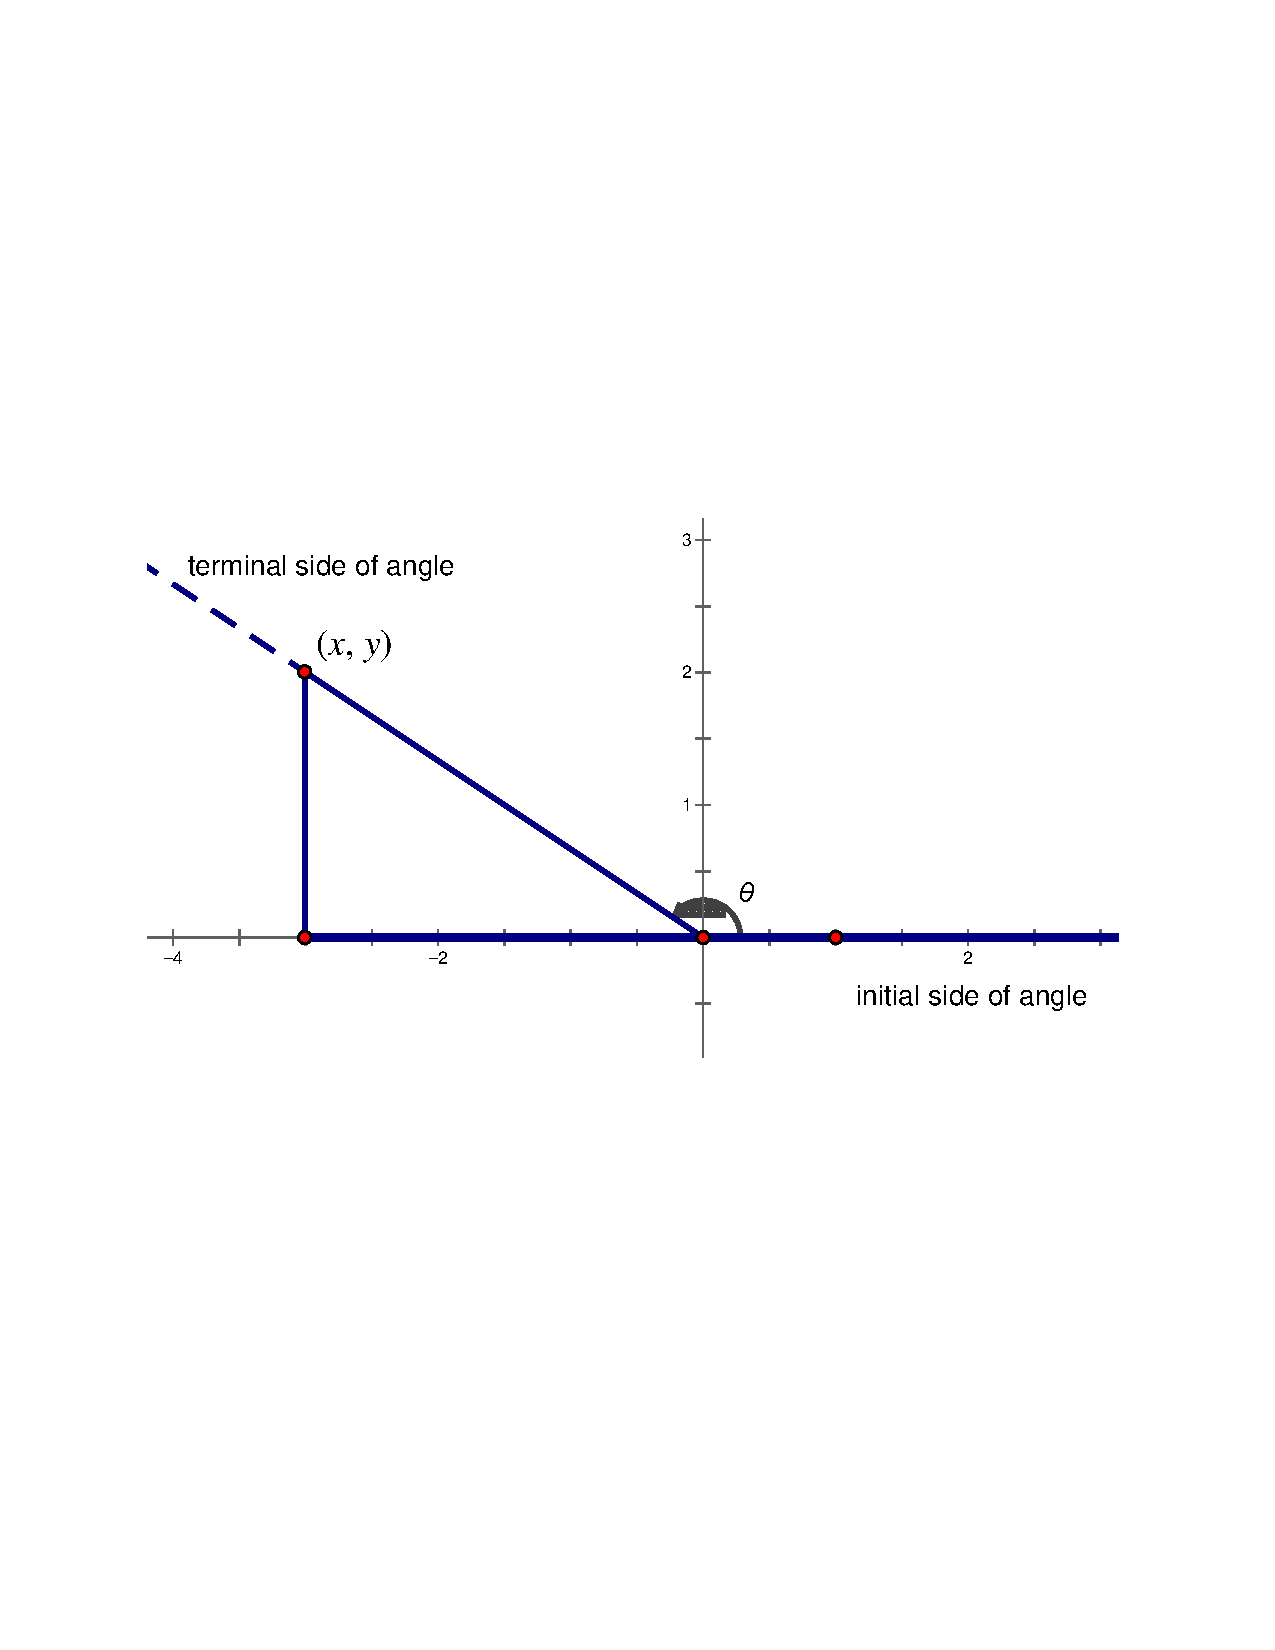
\includegraphics[scale=0.6]{../graphics/referenceTriangle}
\]

If we choose a point on the terminal side of this angle, we can draw what is called \emph{reference triangle} by dropping a perpendicular to the $x$-axis.  Then we can use the values of $x$, $y$, and $r$ from this triangle, just as before.  What is different this time is that $x$ is negative, as will be the case for any angle with a terminal side in the second quadrant.  


\begin{prob}
Draw a picture to demonstrate the following: 
\begin{enumerate}
\item $\sin 135^\circ = $
\item $\cos 135^\circ =$
\item $\tan 135^\circ =$
\end{enumerate}
\end{prob}

\begin{prob}
Draw a picture to demonstrate the following: 
\begin{enumerate}
\item $\sin 150^\circ =$
\item $\cos 150^\circ =$
\item $\tan 150^\circ =$
\end{enumerate}
\end{prob}

\begin{prob}
For some angles, the reference triangle is not actually a `triangle,' but that's okay.  Draw pictures to demonstrate the following: 
\begin{enumerate}
\item $\sin 90^\circ =$
\item $\cos 90^\circ =$
\item $\tan 90^\circ =$
\item $\sin 180^\circ =$
\item $\cos 180^\circ =$
\item $\tan 180^\circ =$
\end{enumerate}
\end{prob}

%\begin{prob}
%Now we can find the area of a triangle given two sides and an angle.\standardhs{G-SRT.9}  
%\end{prob}
%
%% Laws of Sines and Cosines \standardhs{G-SRT.10}, \standardhs{G-SRT.11}

Because angles are often about rotation, angles greater than $180^\circ$ can make sense, too.  And negative angles can describe rotation in the opposite direction.  If we consider the angle to change continuously, then rotation about the origin creates a situation that repeats every $360^\circ$.  This repetition provides the foundation for modeling lots of repetitive (periodic) contexts in the real world.  For this modeling, we need \emph{circular trigonometry}, which turns out to be much cleaner if (1) angles are measured not in degrees but in a more ``natural'' unit, called radians; and (2) we use \emph{the unit circle}, which is a circle of radius 1 centered at the origin.   

\begin{prob}
Below is the unit circle with special angles labeled in degrees, radians, and with coordinates.\standardhs{F-TF.2} 
$$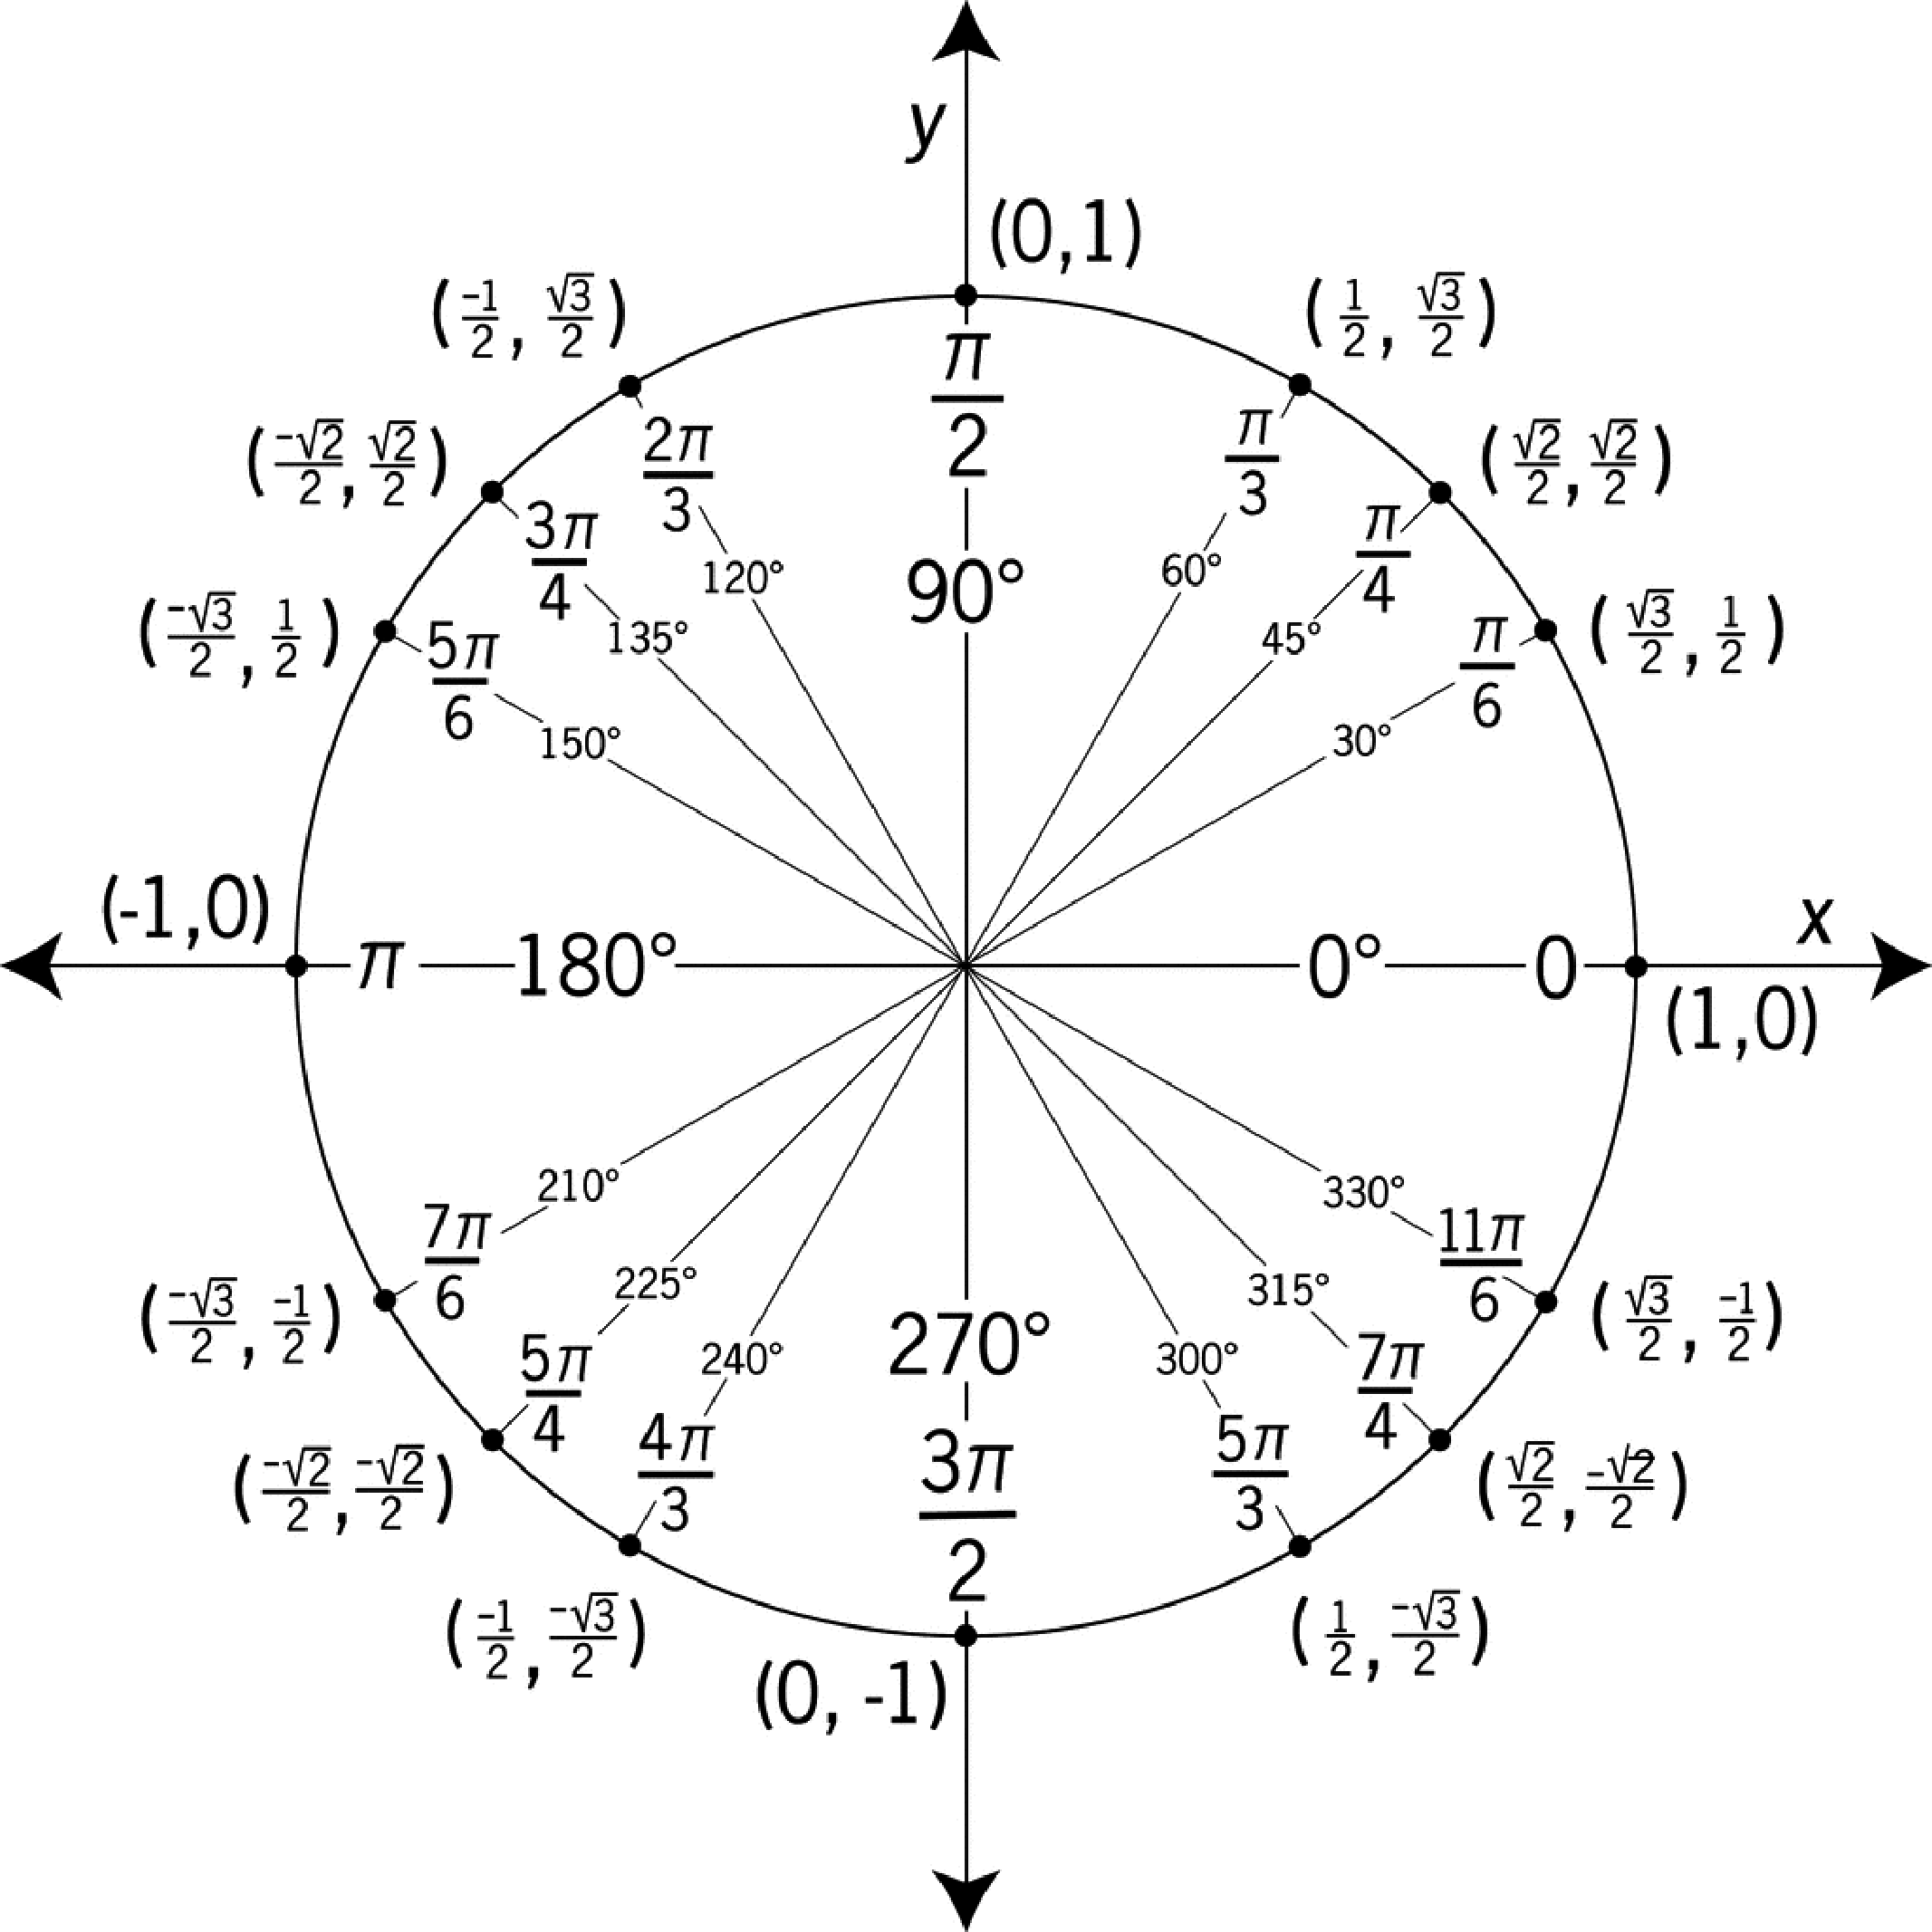
\includegraphics[scale=0.25]{../graphics/unitCircle}$$
\begin{enumerate}
\item Explain what the various numbers mean in this unit circle.  
\item Use the unit circle to make a table showing (1) angle in degrees, (2) angle in radians, (3) sine of the angle, and (4) cosine of the angle.  
\item Use your table to draw a graph of $\sin\theta$ versus $\theta$.
\item Use your table to draw a graph of $\cos\theta$ versus $\theta$.
\item Explain why it makes sense to connect the dots. 
\item Extend your graphs to angles greater than $360^\circ$, and use the unit circle to explain why your extension makes sense. 
\item Extend your graphs to angles less than $0^\circ$, and use the unit circle to explain why your extension makes sense.
\end{enumerate}
\end{prob}

%\begin{enumerate}
%\item Understanding radian measure.\standardhs{G-C.5}, \standardhs{F-TF.1}
%
%\item Using the unit circle to extend trigonometry to angles of any measure.\standardhs{F-TF.2}
%
%\item Choosing and using trig functions to model periodic phenomena.\standardhs{F-TF.5}
%\item Fluency finding trig functions of special angles in radian measure.\standardhs{F-TF.3}
%
%\end{enumerate}

\fixnote{Possibly add an activity with questions about radian measure and modeling with trig functions.}


%\newpage

\section{Quadrilateral Diagonals}
\begin{teachingnote}
Supplies:  Fettuccini, scrap paper, 12-inch rulers.
\end{teachingnote}

Imagine you are working at a kite factory and you have been asked to design a new kite.  The kite will be a quadrilateral made of synthetic cloth, and it will be formed by two intersecting rods that serve as the diagonals of the quadrilateral and provide structure for the kite.  

\begin{prob}
To get started, review the definitions of all special quadrilaterals.  Be sure to include \emph{kite} on your list.  
\end{prob}

\begin{prob}
To consider the possible kite shapes, your task is to describe how conditions on the diagonals determine the quadrilateral.  Use fettuccine to model the intersecting rods, and use paper and pencil to draw the rod configurations and resulting kite shapes.  

Here are some hints:  

\begin{itemize}
\item Explore diagonals of various lengths, of the same length, and of different lengths.  
\item Explore various places at which to attach the diagonals to each other, including at one or both of their midpoints.  
\item Explore various angles that the diagonals might make with each other at their intersection, including the possibility of being perpendicular.  
\item Indicate what kinds of rotational or reflection symmetry you see in the resulting figure.
\end{itemize}
\end{prob}

\begin{prob}
Summarize your findings in a table organized like the one on the next page.  
\end{prob}

\newpage 

{
\renewcommand\arraystretch{2.8}
\renewcommand\tabcolsep{12pt}
\begin{table}[h]
\begin{tabular}{|l|p{6cm}|c|c|c|p{8cm}|}
\hline 
 &   & \multicolumn{3}{c|}{Diagonals} &  \\  %\hline
Quadrilateral & Definition (A quadrilateral with \dots) & \begin{sideways}Cong.\end{sideways} & 
\begin{sideways}Bisect\end{sideways} & \begin{sideways}Perp.\end{sideways} & Comments (e.g., symmetry, other properties) \\ \hline\hline
Square           &            &   &  &         &                  \\  \hline
Rectangle       &           &   &  &         &                  \\ \hline
Rhombus        &           &   &  &         &                  \\ \hline
Parallelogram &           &   &  &         &                  \\ \hline
Kite                &           &   &  &          &                  \\ \hline
Trapezoid       &           &   &  &         &                  \\ \hline
Isosceles Trapezoid       &           &   &  &         &                  \\ \hline
\end{tabular}
\end{table}
}




  % replace other version
%\newpage

\section{Lines in Triangles}
\begin{teachingnote}
This preactivity for Isosceles Bisectors is about (1) the meanings of median, altitude, angle bisector, and perpendicular bisector; (2) drawing them carefully with protractor and ruler; and (3) noticing that they are four different lines in a general triangle. 
\end{teachingnote}

Two copies of a triangle are shown below.   In each triangle, \textbf{draw carefully} the designated lines.  \emph{Construction is not necessary:  careful measurements are allowed.}

\begin{prob}
In the triangle on the left, draw the median from $B$ to $\overline{AC}$, the altitude from $B$ to $\overline{AC}$, the angle bisector of $\angle B$, and the perpendicular bisector of $\overline{AC}$.  

%\begin{enumerate}
%\item Median from $B$ to $\overline{AC}$
%\item Altitude from $B$ to $\overline{AC}$
%\item Angle bisector of $\angle B$
%\item Perpendicular bisector of $\overline{AC}$
%\end{enumerate}
\end{prob}

\begin{prob}
In the triangle on the right, draw the median from $C$ to $\overline{AB}$, the altitude from $C$ to $\overline{AB}$, the angle bisector of $\angle C$, and the perpendicular bisector of $\overline{AB}$. 

%\begin{enumerate}
%\item Median from $C$ to $\overline{AB}$
%\item Altitude from $C$ to $\overline{AB}$
%\item Angle bisector of $\angle C$
%\item Perpendicular bisector of $\overline{AB}$
%\end{enumerate}
%
\end{prob}

\begin{prob}
In each triangle, you should have drawn four different lines.  What might you say about a triangle for which two or more of these lines turn out to be the same?  
\end{prob}

\vfill
\begin{fullwidth}
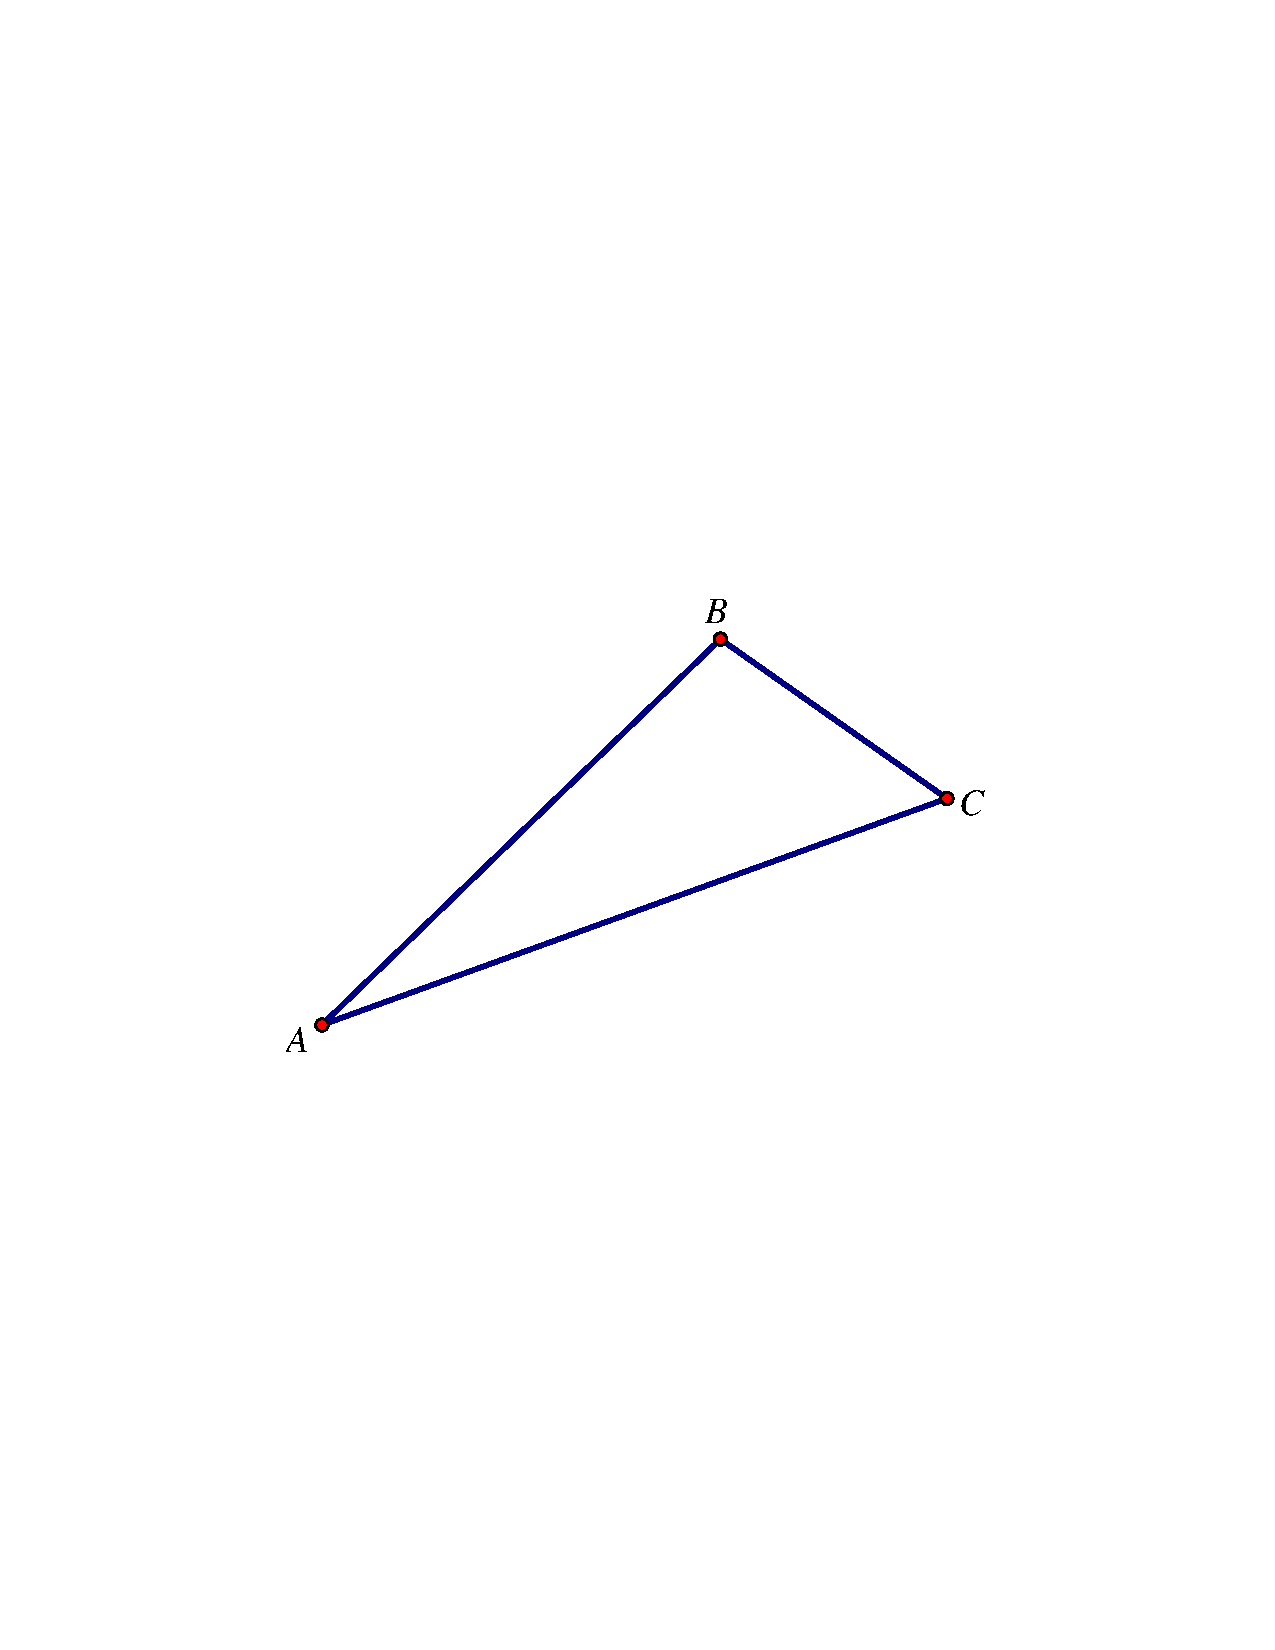
\includegraphics[scale=0.9]{../graphics/obtuseTriangle.pdf}
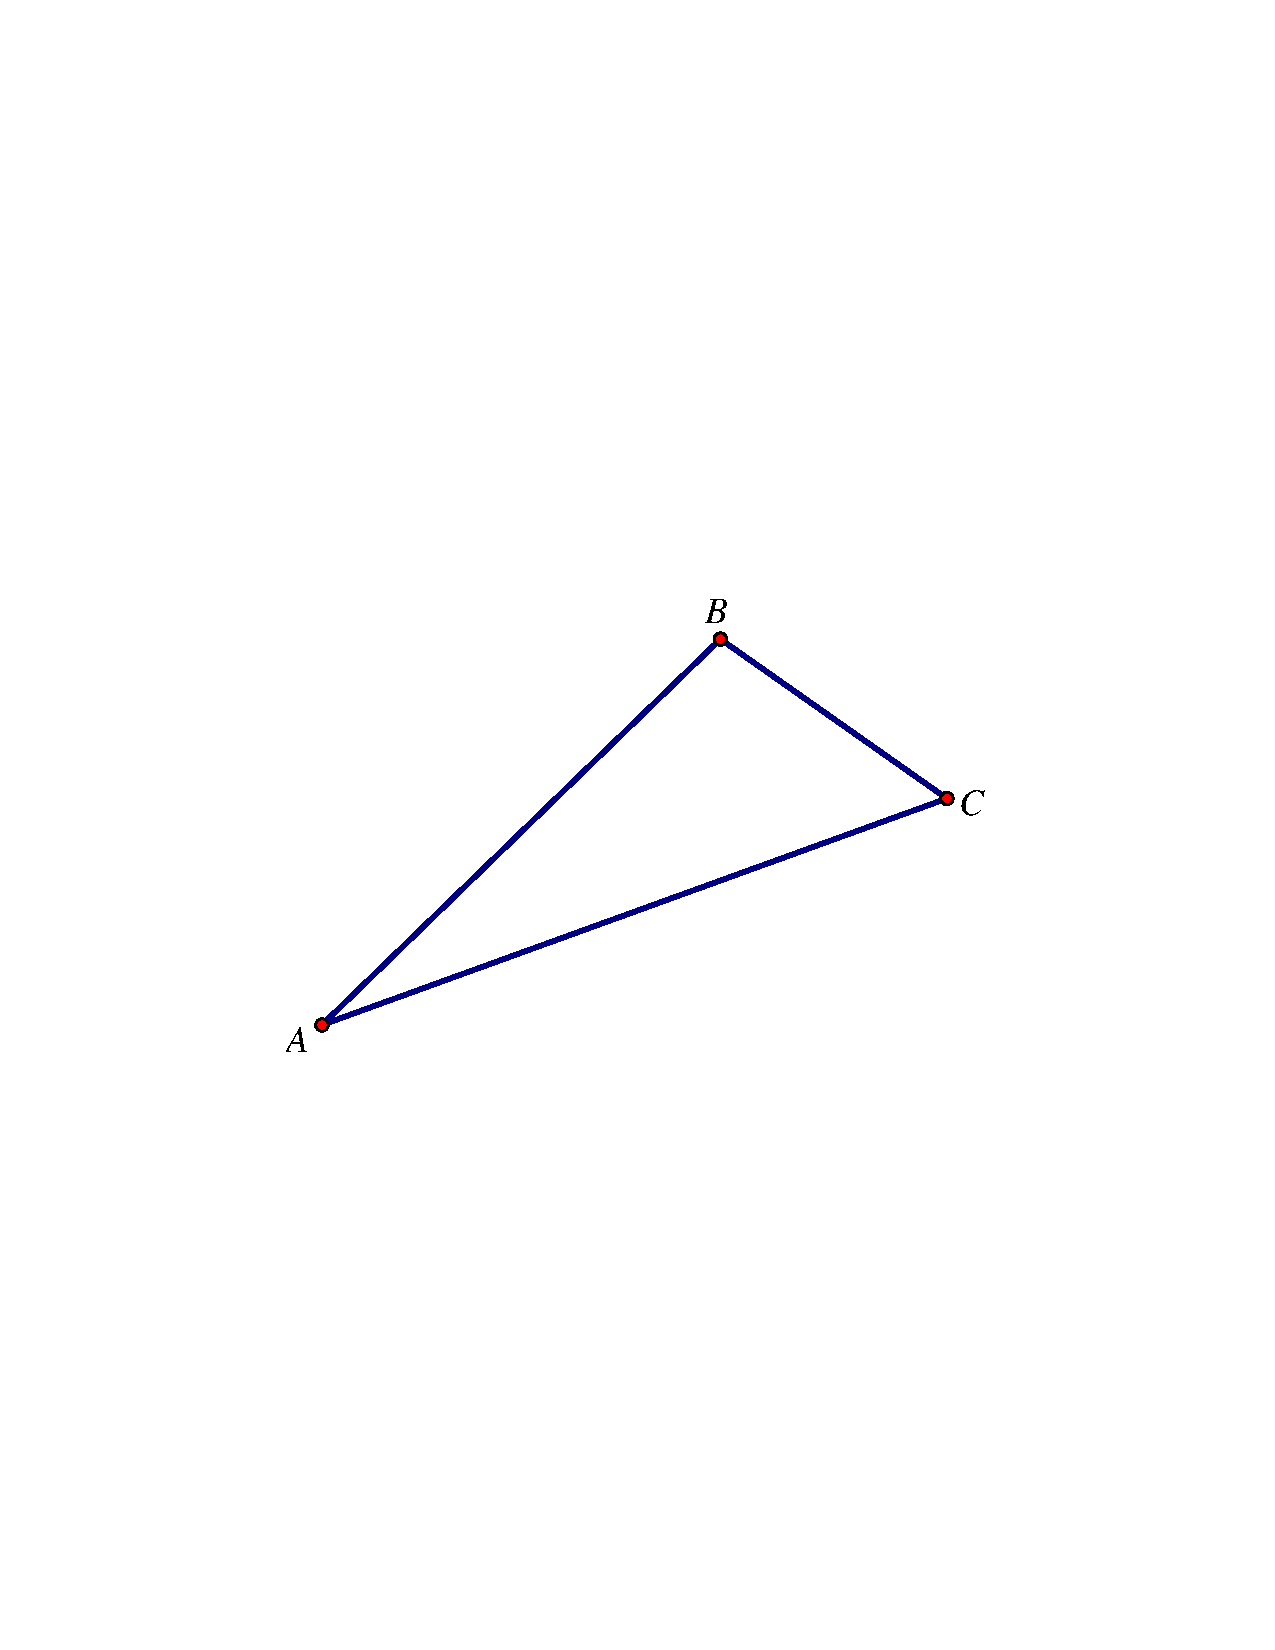
\includegraphics[scale=0.9]{../graphics/obtuseTriangle.pdf}
\end{fullwidth}

\vfill


%\newpage
\section{Constructible Numbers, Part 2}

\begin{prob}
Suppose you are given points $(h, k)$, and $(p, q)$ with integer coordinates?  
\begin{enumerate}
\item Write an equation of the circle with center $(h, k)$ and containing the point $(p, q)$?  
\item What arithmetic operations were involved in writing your equation of the circle?  
\item What can you conclude about the numbers that are coefficients in your equation?   
\end{enumerate}
\end{prob}

\begin{teachingnote}
Finding the intersection of a circle and a line involves a substitution and then solving a quadratic equation:  rational operations and extracting square roots.  

Finding the intersection of two circles involves first subtracting the two circle equations to remove all squared terms.  Then we have a line.  

Our students might not have enough experience with these skills.  
\end{teachingnote}

\begin{prob}
Solve the following equations simultaneously
$$(x-3)^2+(y-2)^2 = 14$$
$$ y = x + 4$$
\end{prob}


\begin{prob}
Solve the following equations simultaneously
$$(x-3)^2+(y-2)^2 = 18$$
$$ y = x + 5$$
\end{prob}

\begin{prob}
Solve the following equations simultaneously
$$(x-3)^2+(y-2)^2 = 12$$
$$ y = x + 4$$
\end{prob}


\begin{prob}
Solve the following equations simultaneously
$$(x-3)^2+(y+2)^2 = 4$$
$$(x-1)^2+(y-2)^2 = 9$$
\end{prob}

\begin{prob}
Solve the following equations simultaneously
$$(x-3)^2+(y+2)^2 = 4$$
$$(x+1)^2+(y-2)^2 = 9$$
\end{prob}


\begin{prob}
Suppose you are given equations of the form 
$$x^2 + ax +y^2+by = c$$
$$x^2 + dx +y^2+ey = f$$
where $a$, $b$, $c$, $d$, $e$, and $f$ are all integers.  
\begin{enumerate}
\item What kind of geometric objects do these equations describe in the $xy$-plane?  
\item What arithmetic operations would you use to solve the equations simultaneously? 
\item What can you conclude about the numbers $x$ and $y$ that are the (simultaneous) solutions of these equations?  
\item How will your answers change if $a$, $b$, $c$, $d$, $e$, and $f$  are all rational numbers?  
\end{enumerate}
\end{prob}

\begin{prob}
Based on the previous problems, if you begin with a coordinate system with only integer coordinates, how would you describe the set of all numbers (coordinates) that are constructible via lines and circles?  
\end{prob}

\begin{prob}
Considering that all compass and straightedge constructions are about lines, circles, and their intersections, what do your results about coordinate constructions imply about compass and straightedge constructions?  
\end{prob}

\begin{prob}
Name some numbers that are \textbf{not constructible} with compass and straightedge.  
\end{prob}



%  Unused activities

%\input{../chapters/appendix/louieRegPoly}
%\input{../chapters/appendix/apothem}
% \input{../chapters/appendix/center}   % Subs at Sea.  Center of an element of a group
%\input{../chapters/appendix/goldenRatio}
%\input{../chapters/appendix/ruleTheDay}


% Figures for Turn Up the Volume!  

\newpage

$$\includegraphics[angle=90,scale=1.2]{../graphics/rightPyramid}$$
\vfill
\newpage

$$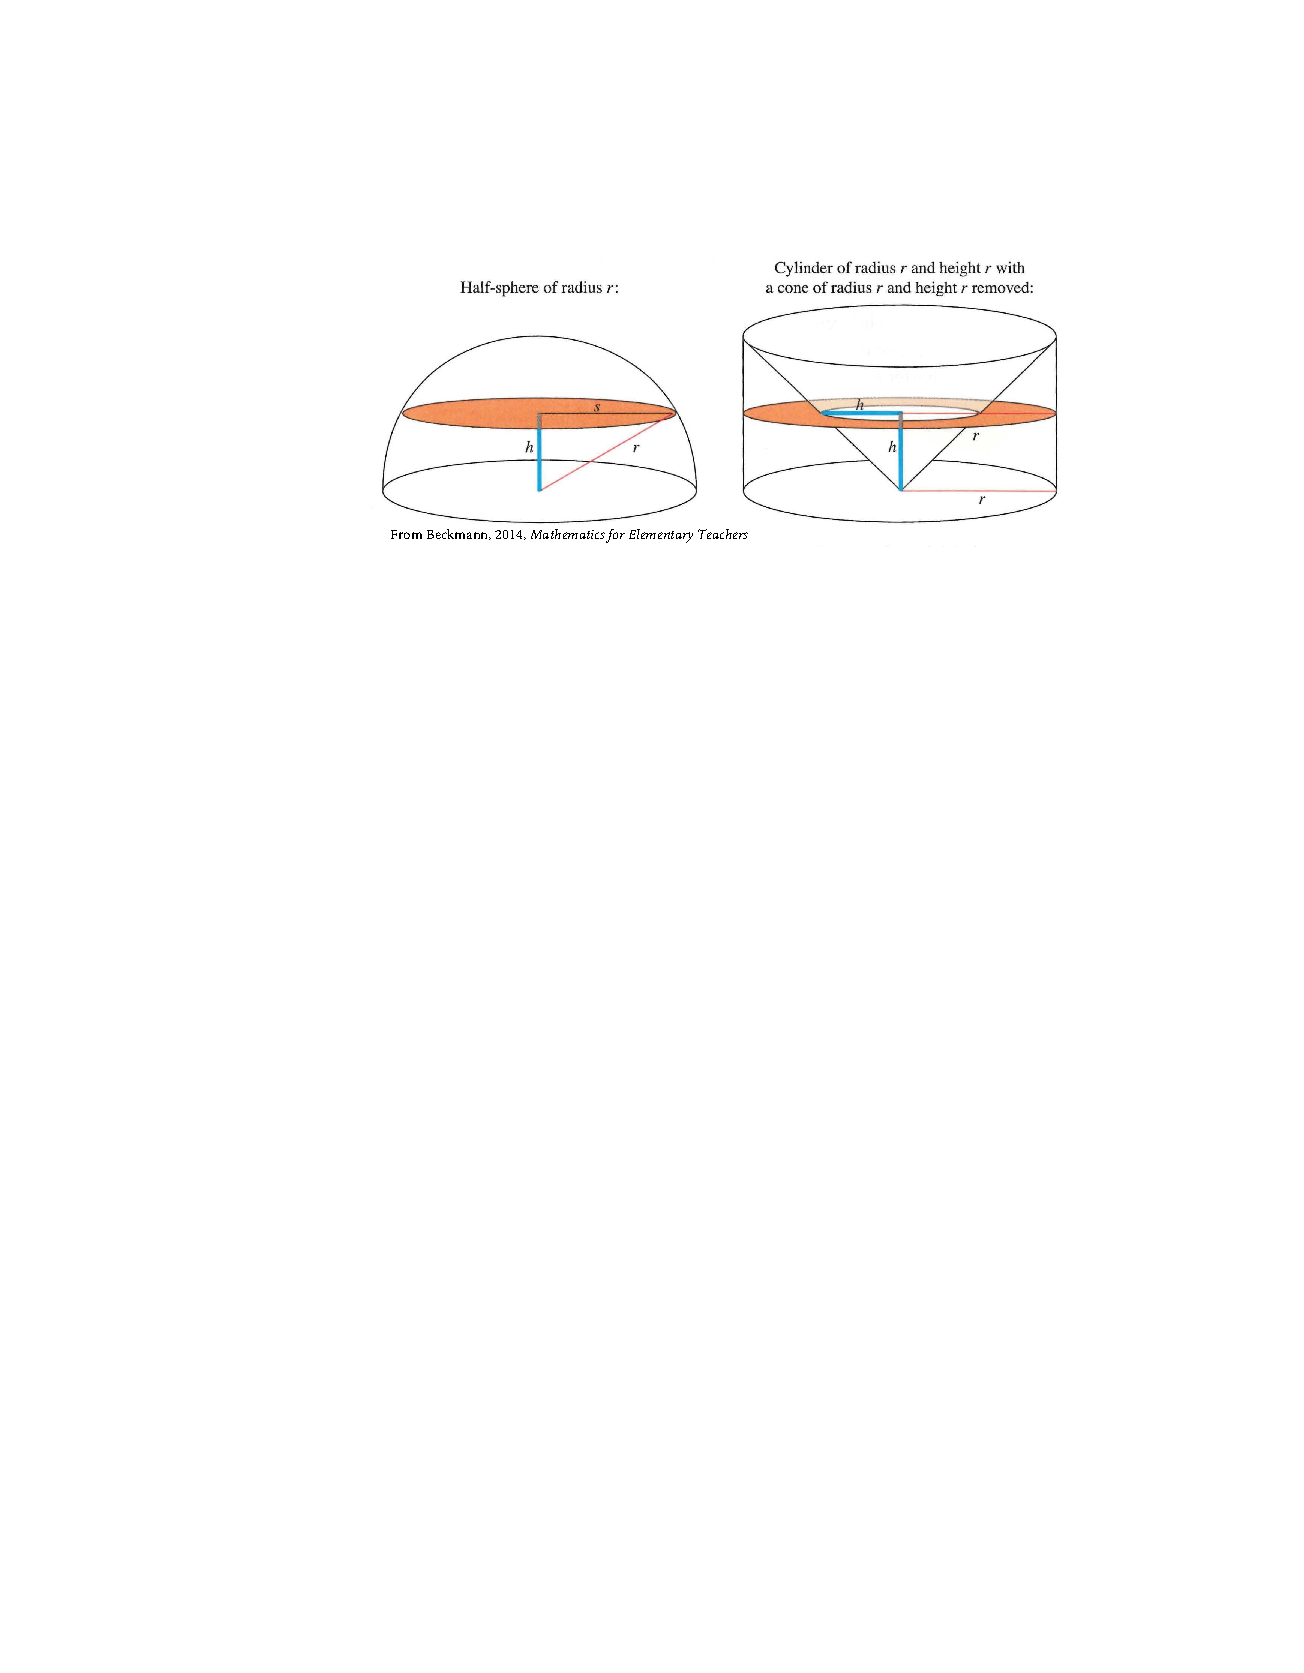
\includegraphics[scale=1.2]{../graphics/sphereVolume}$$

\chapter{Supplemental Problems}
\newpage

\section{Midterm 1 Review, Spring 2022}
Midterm Exam 1 will cover Chapters 1 -- 3 (except section 1.2 and the angle trisection part of 3.1) and activities 1 -- 18, some of which are on the schedule for this week.  We did not complete all of these activities in class so you will need to fill in some gaps.  
\subsection{Review Ideas}

\begin{itemize}\itemsep0em
\item Be able to state definitions of commonly used terms, such as 
\begin{itemize}
\item Perpendicular line, parallel line, line segment, ray, angle, circle
\item Concurrent, collinear
\item Equilateral, equiangular, and regular polygons
\item Acute, obtuse, and right angles and triangles; isosceles and scalene triangles
\item Straight, complementary, and supplementary angles
\item Trapezoid (inclusive and exclusive), parallelogram, rhombus, rectangle, square, kite
\item Median, perpendicular bisector, angle bisector, altitude
\item Centroid, circumcenter, incenter, orthocenter
\item Chord, arc, arc measure, central angle, inscribed angle, tangent
\end{itemize}
\item Be able to perform standard constructions and explain why they work. 
\item Be able to draw (careful) figures satisfying particular conditions.  
\item Be able to explain key concepts such as area and angle.   
\item Be able to state precisely the triangle congruence criteria. 
\item Know the properties of various special quadrilaterals and be able to prove them.  
\item Know the various centers of a triangle, how to construct them, and whether they can lie outside the triangle.  
\item Be able to state key theorems and prove them in at least two (2) ways, especially:  
\begin{itemize}
\item Isosceles triangle theorem and its converse
\item Pythagorean theorem and its converse
\item The angle sum of a triangle 
\end{itemize}
\end{itemize}

\subsection*{Review Problems}
\begin{prob}
Demonstrate and describe Euclid's (compass and straightedge) construction for an equilateral triangle.  Explain
why it works.\marginnote{What about a square or a regular hexagon?}
\end{prob}

\begin{prob}
Maddie had an idea for proving that the sum of the interior angles in a triangle is $180^\circ$:  Given $\triangle ABC$, draw a line through $C$ parallel to $\overline{AB}$.  Finish Maddie's proof.\marginnote{What were the approaches we used in class?}  
\[
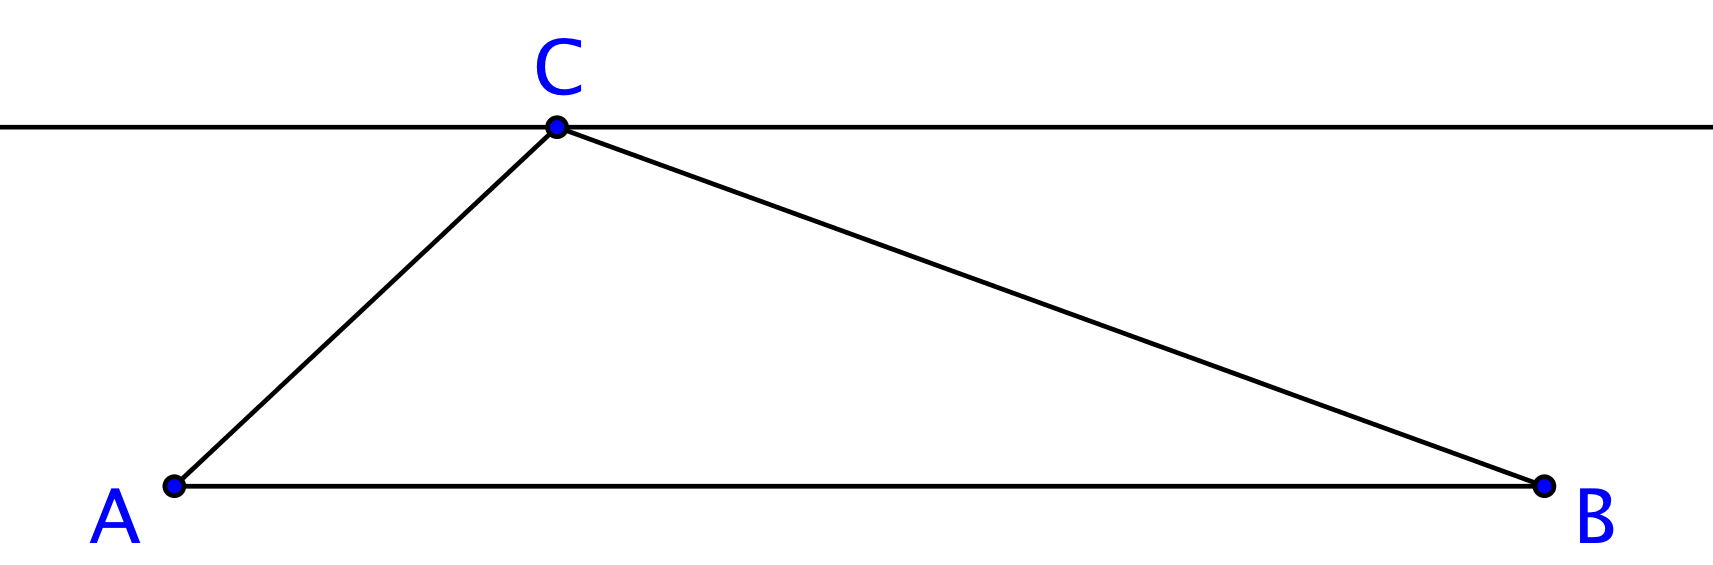
\includegraphics{../graphics/triangleAngleSum.png}
\]
\end{prob}

\begin{prob}
Use the picture below to show that a pair of medians intersects at a point 2/3 of the way from the vertex to the opposite side.  Then use that fact to argue that the three medians must be concurrent.
\[
\includegraphics[width=2.5in]{../graphics/median1.pdf}
\]
\end{prob}

\begin{prob}
Prove that the points on an angle bisector are \emph{exactly those} that are equidistant from the sides of the angle.\marginnote{What about the perpendicular bisectors?}
\end{prob}

\begin{prob}
Prove that the perpendicular bisectors of a triangle are concurrent.\marginnote[\baselineskip]{What about the angle bisectors?}
\end{prob}

\begin{prob}
Construct a $30$-$60$-$90$ right triangle. Explain the steps in your
 construction and how you know it works.\marginnote{What about a $45$-$45$-$90$ triangle?}
\end{prob}

%\begin{prob}
%Construct a $45$-$45$-$90$ right triangle. Explain the steps in your
%  construction and how you know it works.
%\end{prob}

\begin{prob}
Where is the orthocenter of a right triangle?  Explain your reasoning.  What about the circumcenter?  Again, explain your reasoning.\marginnote{What about the other centers of a right triangle?}
\end{prob}

\begin{prob}
Show that, given any three non-collinear points in the Euclidean plane, there is a unique circle passing through the three points.\marginnote{What about four points?}
\end{prob}

\begin{prob}
Construct a tangent line from a point outside a given circle to the circle.
\end{prob}

\begin{prob}
Give an informal derivation of the relationship between the circumference and area of a circle. 
\end{prob}

\begin{prob}
Complete the following statement:  When a quadrilateral is inscribed in a circle, opposite angles are \dots. 
Now prove the statement.  
\end{prob}

\begin{prob}
Claim:  A radius that is perpendicular to a chord bisects the chord.
\begin{enumerate}
\item Prove the claim.\marginnote{Use this problem structure for other problems.}
\item State the converse of the claim. 
\item Is the converse true?  If not, give a counterexample.  
\item If the converse is true, prove it.  If the converse is false, ``salvage it'' to make a true statement, and prove it.
\end{enumerate}
\end{prob}

\begin{prob}
State and prove the isosceles triangle theorem.\marginnote{What about the converse?}
\end{prob}

\begin{prob}
State and prove the Pythagorean theorem.\marginnote{What about the converse?}
\end{prob}

\begin{prob}
Prove any one of the following theorems about quadrilaterals.  State the converse of the theorem (regarding quadrilaterals).  If the converse is true, prove it.  If the converse is false, give a counterexample.  
\begin{enumerate}
\item Opposite sides of a parallelogram are congruent.
\item The diagonals of a rhombus are perpendicular.
\item The diagonals of a rectangle are congruent.
\item The diagonals of a parallelogram bisector each other.
\end{enumerate}
\end{prob}

\begin{prob}
Given a circle, describe a construction that finds its center.  Explain why it works.  
\end{prob}

\begin{prob}
Draw an arbitrary convex quadrilateral.  Form a second quadrilateral by connecting the 
midpoints of the sides of the first quadrilateral.  You will find that the second quadrilateral 
is a special quadrilateral.  Make a conjecture about the second quadrilateral and prove it.  
\end{prob}

%\begin{prob}
%The following picture shows a triangle that has been folded
%  along the dotted lines:
%\[
%\includegraphics{../graphics/origamiPBPTri.pdf}
%\]
%Explain how the picture ``proves'' the following statements:
%\begin{enumerate}
%\item The interior angles of a triangle sum to $180^\circ$. 
%\item The area of a triangle is given by $bh/2$. 
%\end{enumerate}
%\end{prob}
%
%\begin{prob}
%The figure below illustrates a construction given an angle $\theta$ and a segment $\overline{AB}$.  Line $\overleftrightarrow{DE}$ is the perpendicular bisector of $\overline{AB}$, and $\overleftrightarrow{BE}$ is perpendicular to $\overrightarrow{BC}$, as marked.  
%\[
%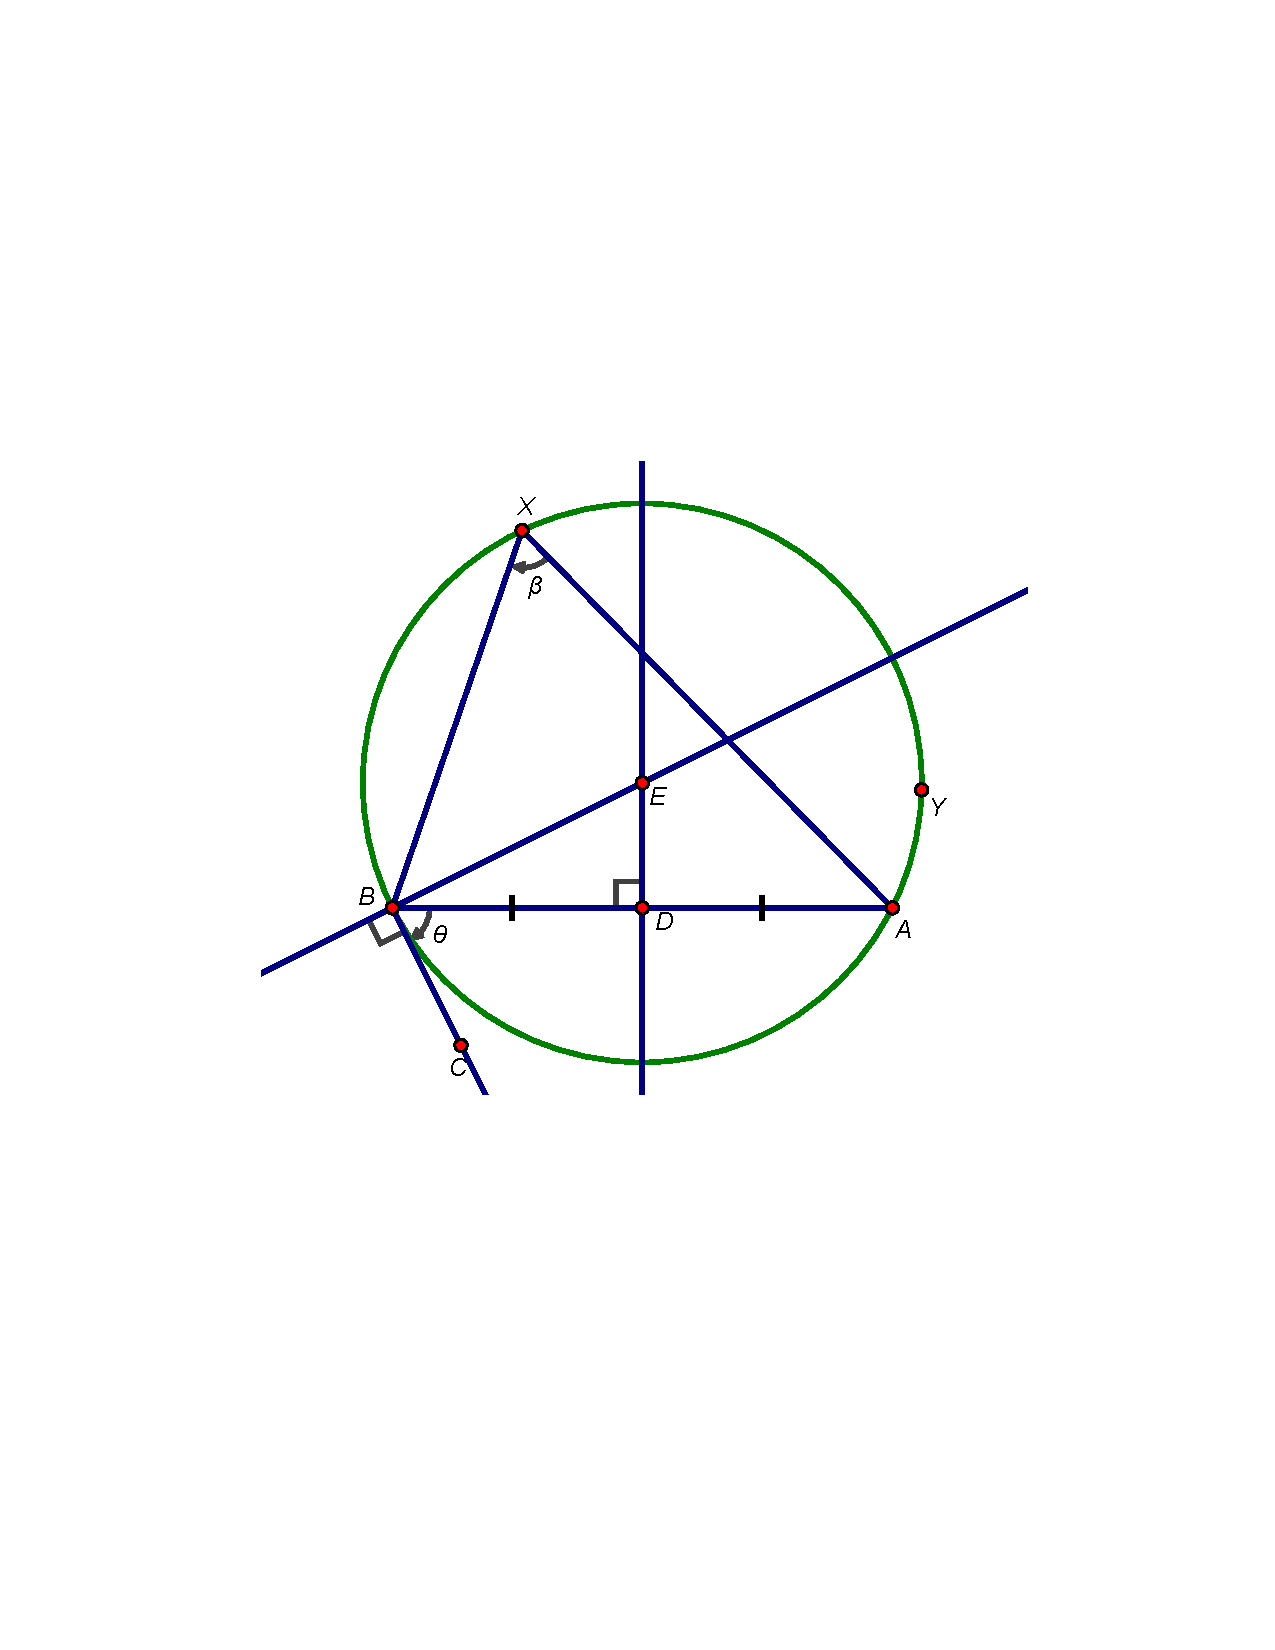
\includegraphics[scale=0.5]{../graphics/trickyConstruction}
%\]
%\begin{enumerate}
%%\item Mark the diagram and state what must be true about the construction so that $\angle\alpha=\angle\beta$. 
%\item Prove that $\angle\theta=\angle\beta$. 
%\item What will happen to $\angle\beta$ if point $X$ is moved over to point $Y$?  Say how you know.  
%\end{enumerate}
%\end{prob}
\newpage

\section{Midterm 2 Review, Spring 2021}

%Midterm 2 will cover Chapter 4, Sections 5.1 and 5.2, Activities A.19--A.35, and A.39. Here are some 

Midterm 2 will cover sections 4.1 through 4.4, Activities A.19--A.32, except trigonometry and the volume ideas in A.32. Here are some specific reminders:
\begin{itemize}\itemsep-3pt
%\item Know the distinction between synthetic and analytic geometry.
\item Know the basic rigid motions, what is required to specify them, and their properties. 
%\item Know what it means to say that transformations of the plane are functions.  
\item Know how to define congruence in terms of basic rigid motions. 
\item Know how to define similarity in terms of dilations and basic rigid motions.  
\item Know and be able to use criteria for congruence and similarity of triangles.  
\item Know how to use transformations  to describe symmetries of figures, including tessellations.  
\item Know the focus and directrix definition of parabola % and be able to use it in both synthetic and analytic geometry.
%\item Know the definition of circle and be able to use it in both synthetic and analytic geometry.
\item Be aware of assumptions underlying Euclidean geometry and how those assumptions can be different in other geometries (such as spherical geometry).  
\item Use similarity to find missing lengths by reasoning from the scale factor or from within-figure comparisons.   
%\item Understand right-triangle trigonometry as similarity, and use trigonometry to solve problems.  (See activity A.27 for a review.)
\item Reason about length, area, and volume in similarity situations.  How are rep-tiles related to this question?  
\item Use shearing and Cavalieri's principle to reason about area. % and volume.  
%\item If you know the area of a rectangle, what can you say about its perimeter?  What about more general figures?  
%\item If you know the perimeter of a rectangle, what can you say about its area?  What about more general figures? 
%\item In coordinate geometry, what is a point?  What is a line?  
%\item Know how to find an equation of the line containing two given points.  
%\item Know how to derive and explain the distance and midpoint formulas. 
\end{itemize}


\subsection{Midterm 2 Review Problems}
Note: Some of the problems below already appear in online homework.

%\begin{prob}
%Ethan stands $120$ feet from the trunk of a tree (along flat ground).  He measures that his line of sight to the top of the tree is at an angle of $53^\circ$ from horizontal.  How tall is the tree?  Explain your reasoning.  
%\end{prob}

\begin{prob}
During a solar eclipse we see that the apparent diameter of the Sun and Moon are nearly equal. If the Moon is around 240,000 miles from Earth, the Moon's diameter is about 2000 miles, and the Sun's diameter is about 865,000 miles how far is the Sun from the Earth?
\begin{enumerate}
\item Draw a relevant (and helpful) picture showing the important points of this problem.
\item Write an expression that gives the solution to this problem---show all work.
\end{enumerate}
\end{prob}

\begin{prob}
David proudly owns a 42 inch (measured diagonally) flat screen
  TV. Michael proudly owns a 13 inch (measured diagonally) flat screen
  TV. Dave sits comfortably with his dog Fritz at a distance of 10
  feet. How close must Michael sit from his TV to have the ``same''
  viewing experience?  Explain your reasoning.
\begin{enumerate}
\item Draw a relevant (and helpful) picture showing the important
  points of this problem.
\item Solve this problem, and be sure to explain your reasoning.
\end{enumerate}
\end{prob}

%\begin{prob}
%Right triangle trigonometry.  
%\begin{enumerate}
%\item Suppose $\alpha$ is in the second quadrant and $\sin\alpha = 3/4$.  Find $\cos\alpha$ and $\tan\alpha$.
%\item Suppose $\beta$ is in the third quadrant and $\cos\beta = -2/3$.  Find $\sin\beta$ and $\tan\beta$.
%\item Suppose $\gamma$ is in the fourth quadrant and $\tan\gamma = -2/3$.  Find $\sin\gamma$ and $\cos\gamma$.
%\end{enumerate}
%\end{prob}

%\begin{prob}
%Right triangle trigonometry: $\alpha$, $\beta$, and $\gamma$ are acute angles.  
%\begin{enumerate}
%\item Suppose $\sin\alpha = 3/4$.  Find $\cos\alpha$ and $\tan\alpha$.
%\item Suppose $\cos\beta = 2/3$.  Find $\sin\beta$ and $\tan\beta$.
%\item Suppose $\tan\gamma = 2/3$.  Find $\sin\gamma$ and $\cos\gamma$.
%\end{enumerate}
%\end{prob}

%\begin{prob}
%Some drugs work best when dosages are proportional to body surface area.  Other drugs work best when dosages are proportional to blood volume.  A typical adult male (5 ft. 10 in.)  has a body surface area of about 2 square meters and about 5 liters of blood.  Scale these values up to estimate LeBron's body surface area and blood volume.  (Recall: LeBron is 6 ft. 8 in. tall.)
%\end{prob}

%\item LeBron James wears size 16 shoe.  Bart says a 5 ft 10 in version of LeBron would have a foot 7/8 as long.  Does this make sense?  Explain why or why not.  If not, give a better estimate.  
%\answer{This is fine because foot length is proportional to height.}
%\item Bart says that the scaled-down LeBron would wear size 14 shoe because 14 is 7/8 of 16.  Does this make sense?  Explain why or why not.  If not, give a better estimate of the scaled version's shoe size.  
%\answer{This is wrong because shoe size is not proportional to foot length.  Somehow suggest that students use Internet data to create a linear function relating foot length to shoe size, and they should get a result close to size 10, which is more sensible.} 

%\begin{prob}
%Consider a version of LeBron that is $d$ times as tall.  How would following quantities compare between the scaled version and the real LeBron:   leather in the sole of a shoe, shoe size, inseam, fabric in a T-shirt, lung capacity, neck circumference, and hat size.\footnote{Cool fact:  The size of a hat is the diameter (in inches) of the hat when it is reshaped into a circle.  Most adults have hat sizes between $6\frac{3}{4}$ and $8$.}  Explain briefly.  
%\answer{\begin{itemize}
%\item Inseam and neck circumference are lengths, so they will be $d$ times as big.  
%\item Hat size is proportional to head circumference, which is a length, so it also scales as $d$.  
%\item Shoe size is not really a length.  It varies with foot length but is not proportional to actual length measurements.  There is a non-proportional linear relationship.  
%\item Leather in the sole of the shoe and fabric in the T-shirt are both about area because their thicknesses stay constant.  They scale as $d^2$.  
%\item Lung capacity is about volume, so it scales as $d^3$.
%\end{itemize}
%}  
%\end{prob}


%\begin{prob}
%A typical adult male gorilla is about 5.5 feet tall and weighs about 400 pounds. Suppose King Kong was about 22 feet tall and proportioned like a typical adult male gorilla.
%\begin{enumerate}
%\item Approximates King Kong's weight. Briefly explain your reasoning.
%\item The circumference of the neck of a typical adult male gorilla is 36 inches. Approximately what would be the circumference of King Kong's neck? Briefly explain your reasoning.
%\item Suppose an Ohio State sweatshirt for a typical adult male gorilla requires 3 square yards of fabric.  Approximately how much fabric would be required for an Ohio State sweatshirt for King Kong?  Briefly explain your reasoning.
%\end{enumerate}
%\end{prob}

%\begin{prob}
%Brenah is drinking fruit punch from a glass shaped like an inverted cone.  Suppose the glass has a height 5 in. and a base of radius 2 in.  What is the volume of the glass?  What is the height of the fruit punch when the glass is half full?  Generalize your result for any glass shaped like an inverted cone.  
%\end{prob}

%\begin{prob}
%A cup has a circular opening, a circular base, and circular cross sections at every height parallel to the base.  The opening has a diameter of 9 cm, the base has a diameter of 6 cm, and the cup is 12 cm high.  
%What is the volume of the cup?  Explain your reasoning.  
%% If the cup is filled to half its height, what fraction of the cup's volume is filled?  Explain your reasoning.  
%\end{prob}

\begin{prob}
Suppose you use a photocopier to enlarge a figure to 125\% of its original size.  What is the scale factor of the enlargement?  What happens to areas under the enlargement?  If you lost the original figure, what reduction percentage would you use on the enlargment to create a figure congruent to the original?  What is the scale factor for the reduction?  
\end{prob}

\begin{prob}
Explain how the following picture ``proves'' the Pythagorean Theorem.
\[
\includegraphics[scale=0.75]{../graphics/pbpdilation.pdf}
\]
\end{prob}

\begin{prob}
Here is a right triangle, note it is \textbf{not} drawn to scale:
\[
\includegraphics{../graphics/origamiSimQ.pdf}
\]
Solve for all unknowns in the following cases.
\begin{enumerate}
\item $a = 3$, $b = ?$, $c = ?$, $d = 12$, $e = 5$, $f = ?$
\item $a = ?$, $b = 3$, $c = ?$, $d =8$, $e = 13$, $f = ?$
\item $a = 7$, $b = 4$, $c = ?$, $d =?$, $e = 11$, $f = ?$
\item $a = 5$, $b = 2$, $c = ?$, $d =6$, $e = ?$, $f = ?$
\end{enumerate}
In each case explain your reasoning.
\end{prob}

\begin{prob}
In a class activity, we established the following Parallel-Side Theorem:  If a line in a triangle is parallel to a side of a triangle, then it splits the other sides of the triangle proportionally. 
$$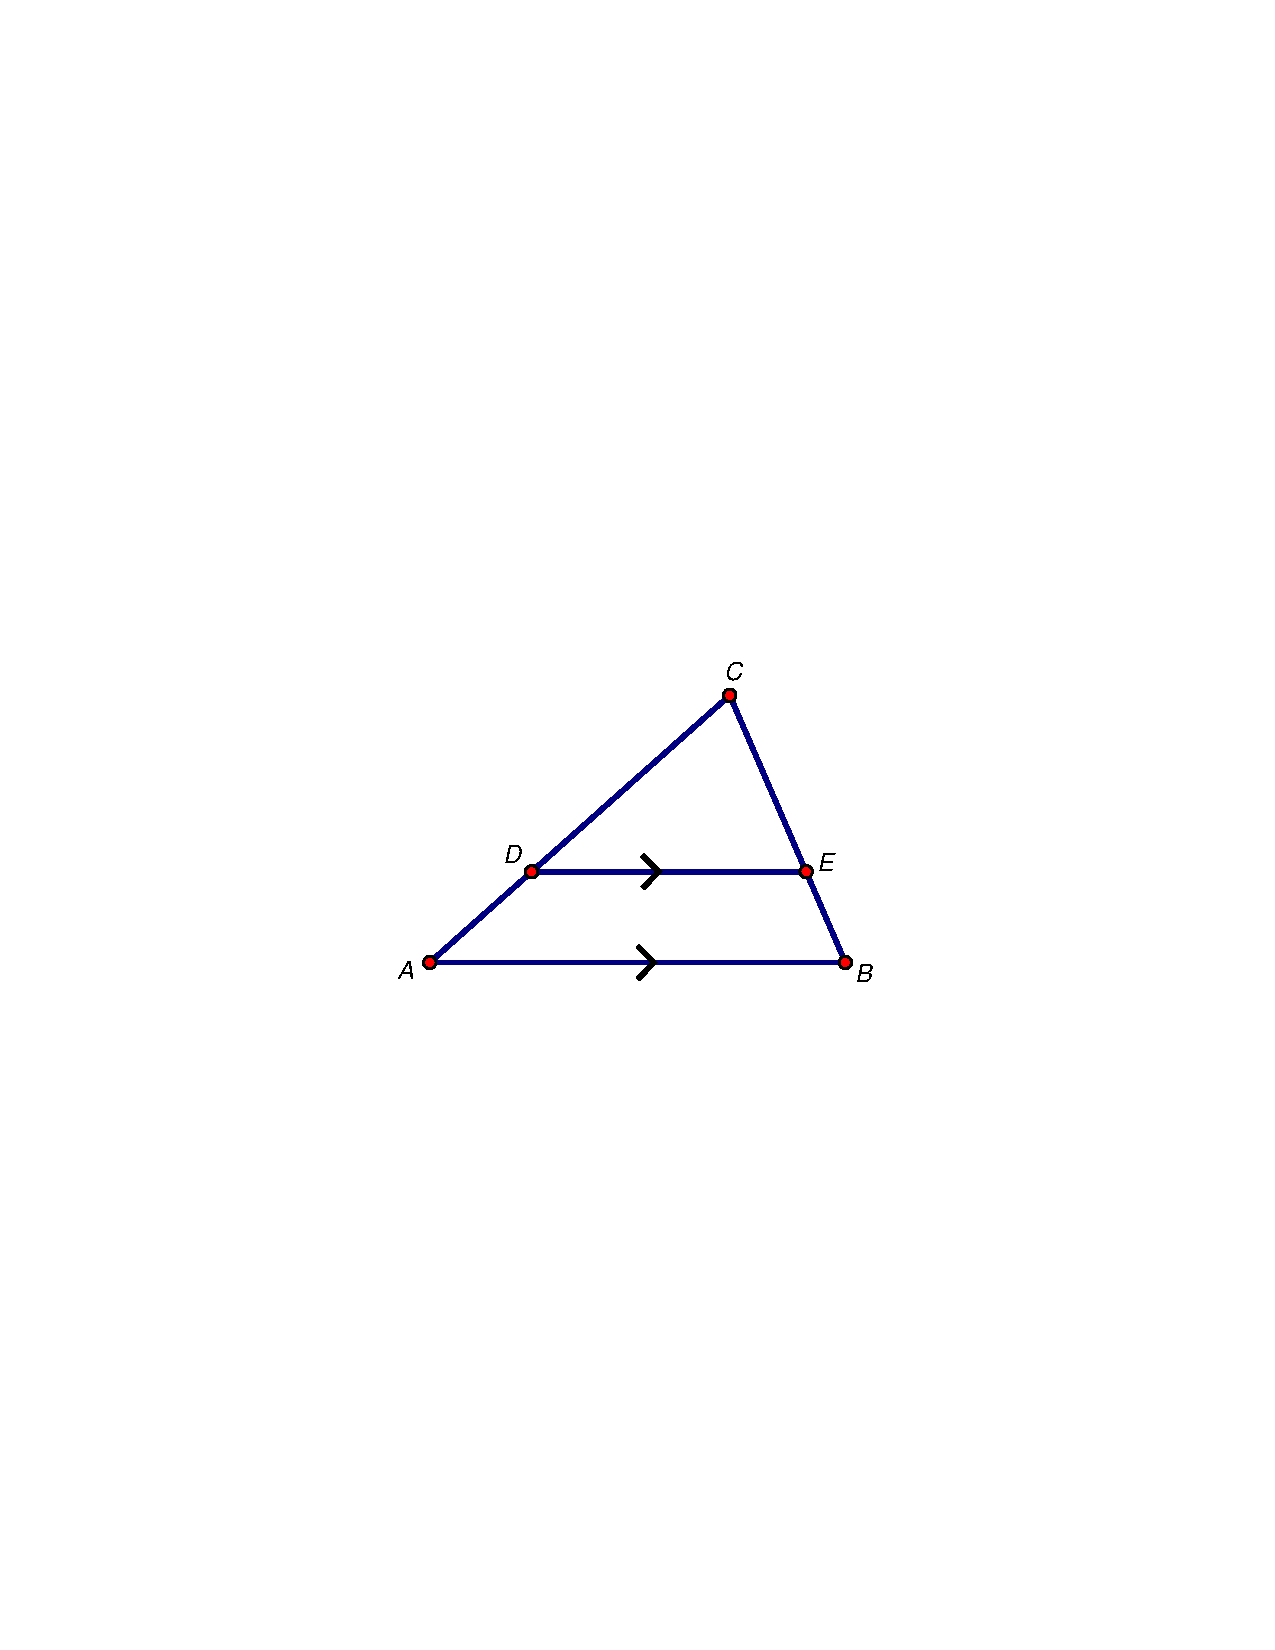
\includegraphics[scale=0.6]{../graphics/Similarity}$$
\begin{enumerate}
\item Using algebra and the Parallel-Side Theorem, you proved that $\frac{AB}{DE}$ is equal to what other ratios?  
%\begin{center}
%$\frac{AB}{DE} = \frac{AC}{DC} =\frac{BC}{EC}$
%\end{center}
\item Explain briefly how the Parallel-Side Theorem implies the AA criterion for triangle similarity.  (Hint: Be sure to use the definition of similarity in terms of basic rigid motions and dilations.)  

\end{enumerate}
\end{prob}

\begin{prob}
The Split-Side Theorem, which is the converse of the Parallel-Side Theorem, is proved in a class activity.   
%(Hint: Using the above figure, draw a line through $D$ and parallel to $\overline{AB}$, 
%and let $X$ be the point where the new line intersects $\overline{BC}$. By the previous results, 
%$\overline{DX}$ divides the sides proportionally. Then argue that $E$ and $X$ must be the same point.)
\begin{enumerate}
\item State the Split-Side Theorem.   (You need not prove it.)
\item Use the Split-Side Theorem to justify the following properties of a dilation given by a center and a scale factor:
\begin{enumerate}
\item A dilation takes a line not passing through the center of the dilation to a parallel line, and leaves a line passing through the center unchanged.
\item The dilation of a line segment is longer or shorter in the ratio given by the scale factor.
\end{enumerate}
\item Explain briefly how the Split-Side Theorem establishes the SAS criterion for triangle similarity.  
\end{enumerate}
\end{prob}

\begin{prob}
Circles, chords, and areas. Find similar triangles in the figure below in order to establish a relationship among the lengths $AX$, $BX$, $CX$, and $DX$.  Explain your reasoning.
%\begin{enumerate}
%\item Find similar triangles in the figure below in order to establish a relationship among the lengths $AX$, $BX$, $CX$, and $DX$.  Explain your reasoning.  
%%$$\includegraphics[scale=0.45]{Secants}$$
$$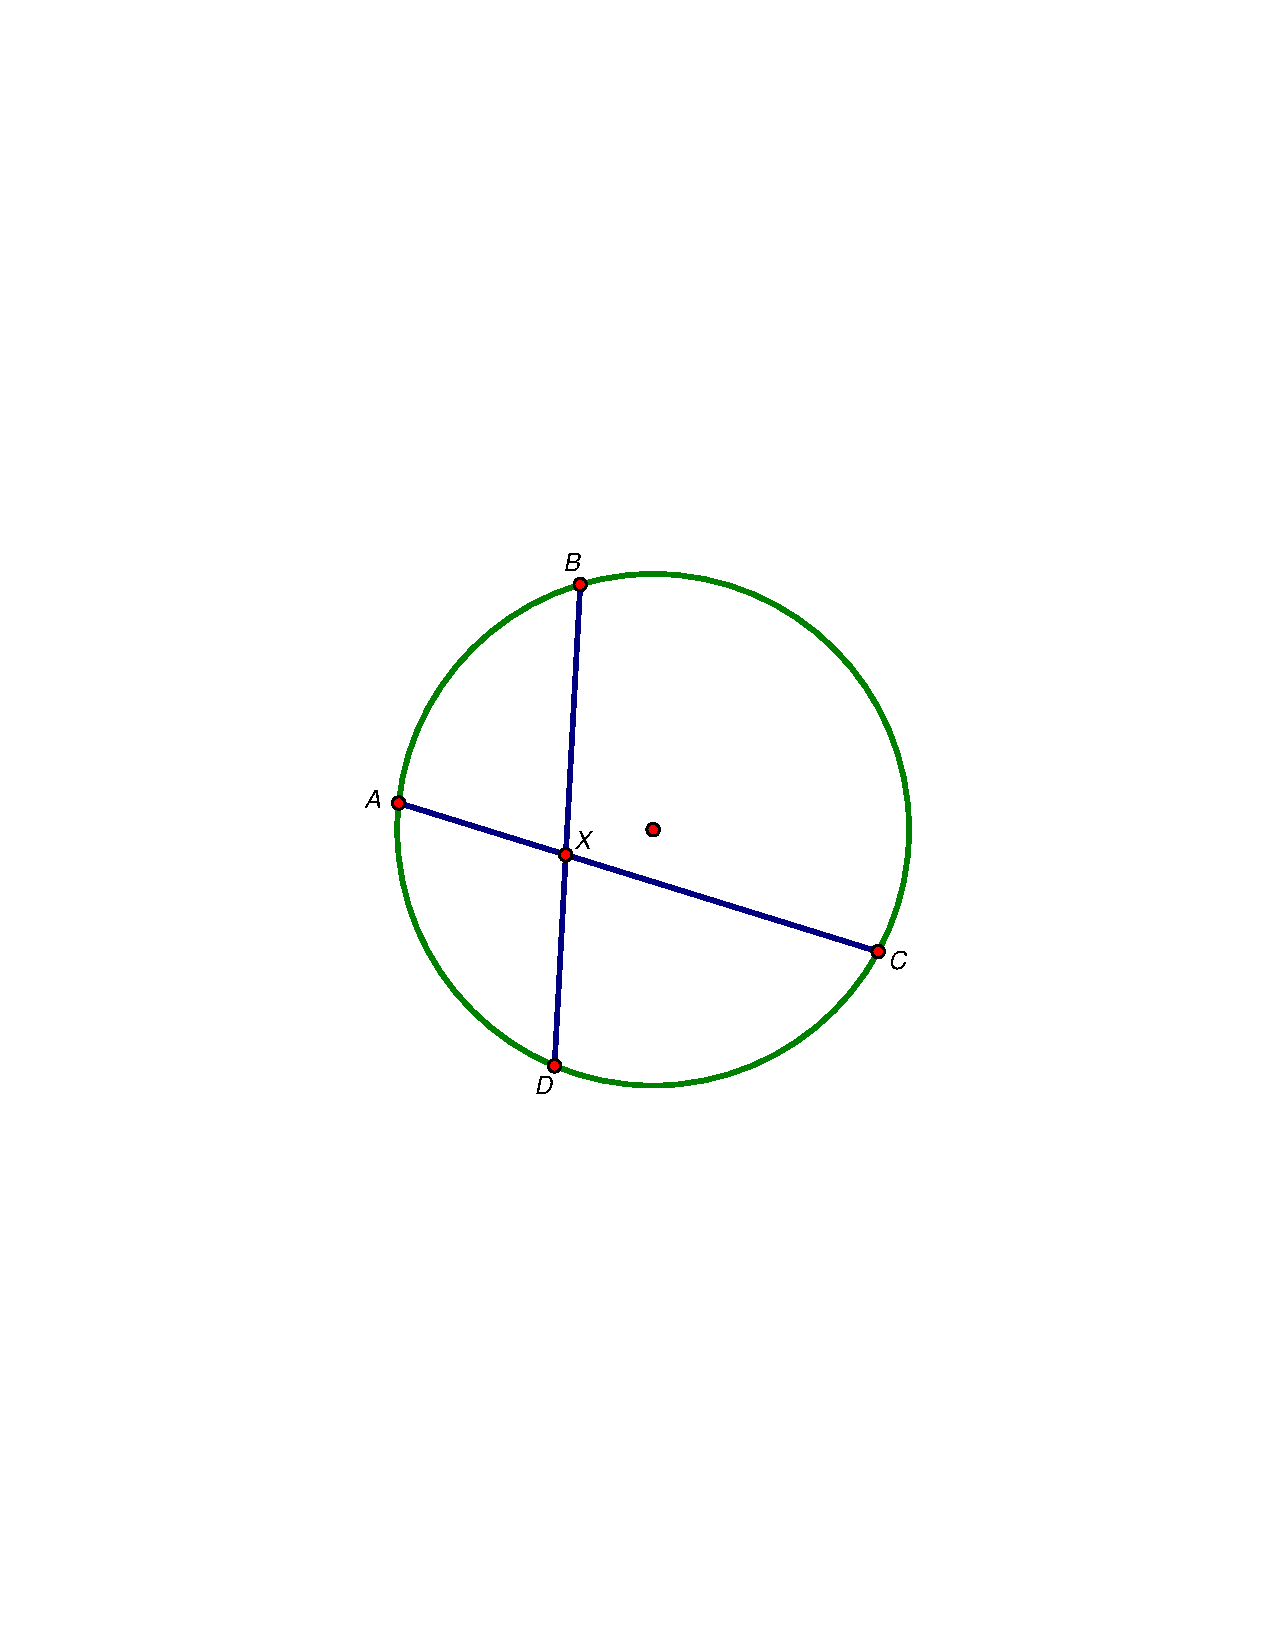
\includegraphics[scale=0.6]{../graphics/CircleChords}$$
%\item Suppose you are given a rectangle with sides of length $a$ and $b$ (and hence area $ab$).  Suppose you are also given a separate segment of length $c$.  Use your result from part (a) to describe how to construct a rectangle with sides $c$ and $x$ so that it has the same area as the rectangle with sides $a$ and $b$. 
%\end{enumerate}
\end{prob}


\begin{prob}
Describe a general (and foolproof) way of demonstrating that any two parabolas are similar.
\end{prob}

\begin{prob}
Prove that for a triangle, the sum of the interior angles is $180^\circ$.
\end{prob}

%\begin{prob}
%Construct a tangent line from a point outside a given circle to the circle.
%\end{prob}
%
%\begin{prob}
%Explain how the formula for the volume of a sphere follows from the formula for the volume of a cone and Cavalieri's Principle.
%\end{prob}
%
\begin{prob}
Give an informal derivation of the relationship between the circumference and area of a circle. 
\end{prob}

\begin{prob}
Given a figure and a rotation of that figure, find the center and angle of rotation.  
\end{prob}
\newpage 

\begin{prob}
In the figure below  $O$ is the center of the circle, $\overline{XY}$ is a diameter, $a = PX$, $b=PY$, and $c=PZ$.  
$$\includegraphics[scale=0.6]{../graphics/means}$$
\begin{enumerate}
\item Show that $c=\sqrt{ab}$.  
\item Use the figure to explain the Arithmetic-Geometric Mean Inequality: $\frac{a+b}{2} \ge \sqrt{ab}$.  
%\item Why is this called the Arithmetic-Geometric Mean Inequality?  
\end{enumerate}
\end{prob}


%\begin{prob}
%If the perimeter of a rectangle is 20 feet, what is the most one can say about the rectangle's area?  If the perimeter of any simple closed 2-dimensional shape is 20 feet, what is the most anyone can say about its area?
%\end{prob}
%
%\begin{prob}
%If the surface area of a rectangular prism is 20 square feet, what is the most one can say about the prism's volume?  If the surface area of any simple closed 3-dimensional shape is 20 square feet, what is the most one can say about its volume? 
%\end{prob}
%
%\begin{prob}
%Why do cute furry animals curl up to stay warm in the winter?  Why are most ugly desert reptiles long and skinny?
%\end{prob}
%
%\begin{prob}Simple closed curve A is contained entirely inside simple closed curve B.  
%\begin{enumerate}
%\item True or False:  The area enclosed by A is less than the area enclosed by B. Explain
%\item True or False:  The perimeter of A is less than the perimeter of B. Explain.  
%\end{enumerate}
%\end{prob}

\begin{prob}
Is it correct to say that ``area is length times width''?  Think about what these three quantities mean.  When would it be correct in the numerical sense and why?  (Make sure you use the meaning of multiplication.)   
\end{prob}

%\begin{prob}
%The apothem of a regular polygon is defined to be the shortest distance from the center of the polygon to an edge.
%\begin{enumerate}
%\item There is a nice relationship between the apothem, perimeter, and area for a regular polygon.  See if you can find it. (Hint:  Split the polygon into congruent triangles from its center and find the area of the polygon in terms of the apothem and perimeter.)  You can assume you know the area of a triangle $=\frac{1}{2}$(Length of Base)(Length of Height).
%\item What does this result say about the area of a circle?  Explain. (Assume you know the circumference of a circle is $2\pi(radius)$.)
%\end{enumerate}
%\end{prob}

%\begin{prob}
% Is it correct to say that ``volume is length times width times height''? What must be true about a figure so that the numerical volume can be more easily measured by ``area times height''?
%\end{prob}
%
%\begin{prob}
%Are there figures for which there is no formula for measuring length, area, and volume?  Explain.  What does your answer to this question imply about the teaching of geometric measurement?
%\end{prob}
%
%\begin{prob}
%Convert 25 yards to meters (and 25 meters to yards) using ``2.54 cm in each inch'' as the only Metric-English unit conversion.  Now convert 25 square yards to square meters and 25 square meters to square yards.  Do the same with cubic yards and cubic meters.
%\end{prob}
%
%\begin{prob}
%In track and field, 1600 meters is often called the ``one mile,'' but this is not exactly correct.  Is 1600 meters longer or shorter than one mile?  By how much?  
%\end{prob}

\begin{prob}
Felicia and Wesley are neighbors.  The common boundary between their properties consists of two line segments, as shown below.  
$$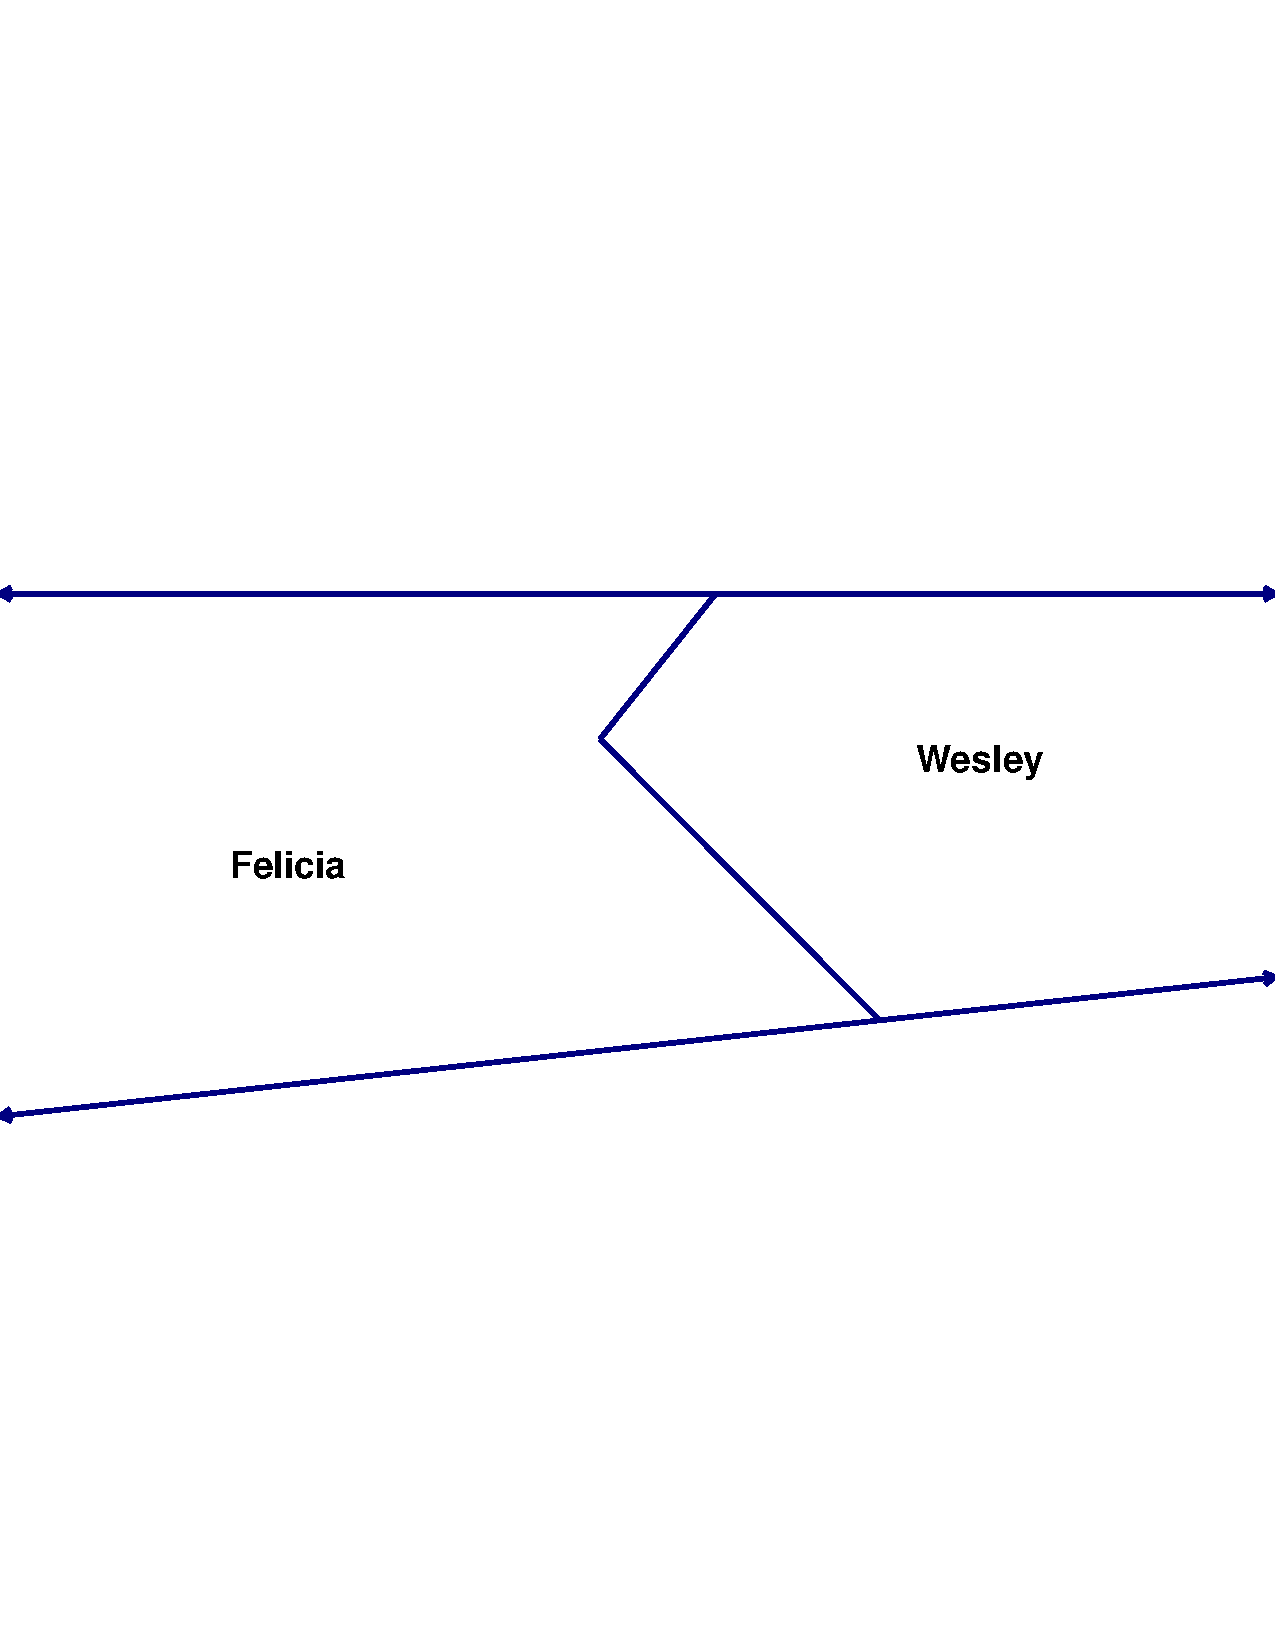
\includegraphics[scale=0.38]{../graphics/TIMSS}$$
They would prefer their common boundary to be a single straight segment.  How might they change their boundary so that they 
each have the same area as they have now?  
\end{prob}

%\begin{prob}
%Write an equation of the line through $(2,4)$ parallel to $5x-3y=1$.  
%Now write an equation of the line through $(x_1,y_1)$ parallel to $ax+by=c$. 
%\end{prob}
%
%\begin{prob}
%Write an equation of the line through $(2,4)$ perpendicular to $5x-3y=1$.  
%Now write an equation of the line through $(x_1,y_1)$ perpendicular to $ax+by=c$. 
%\end{prob}
%
%\begin{prob}
%Intersections of lines.  
%\begin{enumerate}
%\item Find the intersection of the lines $2x-3y=4$ and $3x-5y=3$.  
%\item Find the intersection of the lines $2x-3y=4$ and $-4x+6y=-8$.
%\item Find the intersection of the lines $2x-3y=4$ and $-4x+6y=5$.
%\item How might you have predicted in advance how many solutions to expect for each previous system of equations?
%\item Use algebra to help explain why lines intersect in zero, one, or infinitely many points.  (You know this geometrically, of course.  Here you demonstrate how algebra gives the same result.)  Indicate clearly the algebraic conditions
%for which you get zero, one, or infinitely many points.  
%\end{enumerate}
%\end{prob}
%
%\begin{prob}
%Suppose you have a rectangle with vertices at $(0,0)$, $(a,0)$,
%$(a,b)$ and $(0,b)$. Use algebra to prove that the diagonals have the
%same length.
%\end{prob}

\begin{prob}
Use a general (non-special) triangle to explain why every triangle is a rep-4-tile.  
Use the same triangle to explain why every triangle tessellates the plane.  Then use your tessellation to explain why every triangle is a rep-$n^2$-tile for any positive integer $n$. 
\end{prob}

%\begin{prob} 
%Concurrency of angle bisectors. 
%\begin{enumerate}
%\item For an arbitrary triangle, draw carefully to demonstrate that the angle bisectors of a triangle are concurrent at the incenter.   
%\item Prove that the angle bisectors of a triangle are concurrent.  (Hint:  You may use the result, proved in lecture, that the points on an angle bisector are exactly those that are equidistant from the sides of the angles.)  
%\end{enumerate}
%\end{prob} 

%\begin{prob}
%Explain how the ASA congruence criterion follows from the definition of congruence in terms of rigid motions. Be sure to indicate, using the two given angles and the included side, why the sequence of rigid motions guarantees triangle congruence.
%\end{prob}

%Other review
% * Multiplication is not necessarily scaling--unless it is dilation
%
% * Use of cavalieri's principle 
% * Volume as Area of base times height.
% * Stacking cubic units covering the base. 



%
\newpage

\section{Math 1166: Final Exam Review, Draft 2019}

Note:  The final exam is cumulative, so be sure to include the \textbf{previous midterm review documents} as part of your review.  
Since the second midterm, we will have covered Sections 5.3, 6.1 and 6.2 from your notes as well as Activities A.36 -- A.49, except A.38 and A.46.  Below is a summary of that content.  

Some of the following problems (as well as a few others) will be part of an online supplementary review, available by Reading Day.  

% A.40.Reading Information from a Graph
% A.41. Parametric Equations
% A.38.  Constructible Numbers (section 5.4) 
% Trig Checkup.  Circular trigonometry
% A.42. Parametric Plots of Circles
% A.44. Taxicab Distance (section 6.1)
% A.43. Eclipse the Ellipse
% A.45. City Geometry and Absolute Value
% A.47. Midsets Abound (section 6.2)
% A.48. Tenacity Paracity

\subsection*{Coordinate Geometry}
\begin{itemize}\itemsep-3pt
\item What are the benefits of the standard form, the point-slope form, and the slope-intercept form of a line?  
\item Find an equation of a line through a given point parallel to a given line.  (Try this in standard form.)  
\item Find an equation of a line through a given point perpendicular to a given line.  (Try this in standard form.) 
\item Given two lines, two circles, or a line and a circle, find their intersection(s) if any.  Describe what is happening geometrically when the algebra yields no solutions, exactly one solution, exactly two solution(s) or infinitely many solutions. 
\item Given an equation of a circle or a parabola, complete the square to find the center of the circle or the vertex of the parabola.  
\item What are constructible numbers?  What are some numbers that are not constructible? 
\end{itemize}

\subsection*{City Geometry}
\begin{itemize}\itemsep-3pt
\item Know the distance formula in city geometry, be able to use it, and explain its meaning. 
\item Given a center and a radius, graph a city-geometry circle and write its equation.  
\item Given two points in city geometry,  graph their midset and write an equation of the midset.  
\item Given a focus and a directrix, graph the city-geometry parabola and write its equation.  
\item Explain the absolute value function in several ways.
\item Graph and analyze absolute value equations (such as equations of city-geometry circles, midsets, or parabolas) by checking cases.  
\end{itemize}

\subsection*{Functions}
\begin{itemize}\itemsep-3pt
\item What is a function?  What do domain and range mean?  
\item Why is ``Is this a function?'' a poor question.  What is a better question?  
\item Graph and analyze parametric equations describing a path in the plane
\item In what sense are transformations of the plane functions?  What are the input and output values?  What are the domain and range of an isometry or dilation of the plane?  
\item Describe and analyze functions involving several related variables, such as length, width, area, and perimeter of rectangles.   When fixing one of these quantities, what kinds of functions can you find among the other quantities? 
\end{itemize}



%\subsection{Parametric Equations}
\subsection{Supplemental Review Problems}
The problems below target content since the second midterm exam. 

\begin{prob} 
Consider a nonzero vector defined by the ordered pair $(a,b)$. Let $m$ be the magnitude (length) of this vector, \textbf{use algebra} to explain why
\[
\frac{(a,b)}{m}
\]
is a new vector whose magnitude is $1$ and whose direction is the same
as $(a,b)$.
\end{prob} 

\begin{prob}
Suppose you have a parametric plot defined by $x(t)$ and $y(t)$.
\begin{enumerate}
\item Compare and contrast the plots of
\[
\bigg(x(t),y(t)\bigg)\qquad\text{and}\qquad\bigg(x(t-6),y(t-6)\bigg).
\]
\item Suppose that there are two bugs whose positions are given by:
\[
\mathrm{bug}_1(t) = \bigg(x(t),y(t)\bigg)\qquad\text{and}\qquad\mathrm{bug}_2=\bigg(x(t-6),y(t-6)\bigg).
\]
where $t$ represents time in seconds. Describe what happens as $t$
runs from $0$ seconds to $36$ seconds.

\item Now suppose that there are two bugs whose positions are given
  by:
\[
\mathrm{bug}_1(t) = \bigg(x(t),y(t)\bigg)\qquad\text{and}\qquad\mathrm{bug}_2=\bigg(x(t)-6,y(t)-6\bigg).
\]
where $t$ represents time in seconds. Describe what happens as $t$
runs from $0$ seconds to $36$ seconds.
\end{enumerate}
\end{prob} 

\begin{prob}
Find the intersection of the lines
\begin{align*}
x_1(t) &= -6 + 9t & x_2(t) &= 3+t \\
y_1(t) &= 3-2t &  y_2(t) &= -4-2t 
\end{align*}
If $(x_1(t),y_1(t))$ gives the position of $\mathrm{jogger}_1$ and
$(x_2(t),y_2(t))$ gives the position of $\mathrm{jogger}_2$, what is
the significance of the point of intersection of these lines, from the
perspective of the joggers?
\end{prob}

\begin{prob}
A bug moves according to the following parametric equations, where t is measured in seconds and $x$ and $y$ are measured in centimeters:  $x = 2t^2$, $y = t-2$.  (Suppose $t$ can be any real number.)   
\begin{enumerate}
\item Describe the path of the bug.  
\item Is the bug's position a function of time?  
\item On the path, is $y$ a function of $x$?  
\item Is $x$ a function of $y$?  
\item If you know one of $x$, $y$, or $t$, can you determine the other two?  How does this question relate to the previous two questions?  
\item In school mathematics, students are often given a graph and asked, ``Is it a function.''  Explain why this is a poor question.  What better questions could you ask?  
\end{enumerate}
\end{prob}

%\subsection{Absolute Value, Distance, and City Geometry}
\begin{prob}
Consider the following equations:  
\setlength{\arraycolsep}{12pt}
\setlength{\extrarowheight}{3pt}
\[
\begin{array}{cccc}
x^2-y^2=0    &   x^2=y^2   &   |y|=|x|   &   y= \pm x \\
(x-y)(x+y)=0  &   x= \pm y   &   y = \pm|x|   & x = \pm|y|
\end{array}
\]
\begin{enumerate}
\item Which equations are equivalent to which other equations?  Say how you know.  (Be sure to state what it means for the equations to be equivalent.)
\item For each set of equivalent equations, graph the solution set, and describe how each of the equations provides a different way about thinking about that solution set.  
\end{enumerate}
\end{prob}

\begin{prob}
Distance formulas and circle equations across dimensions.  
\begin{enumerate}
\item What is the (Euclidean) distance formula in 2 dimensions, on the $xy$-plane?  
\item What is the distance formula in 3 dimensions?
\item What is the distance formula in 1 dimension?
\item Write an equation of the circle of radius $r$ and center $(a, b)$.  
\item Explain how a circle is a one-dimensional figure living in a two-dimensional ``space.''
\item In three-dimensional space, write an equation of the two-dimensional ``circle'' of radius $r$ and center $(a, b, c)$.  
\item In one-dimensional space, write an equation of the zero-dimensional ``circle'' of radius $r$ and center $a$.  
\end{enumerate}
\end{prob}

%\begin{prob}
%Distances across dimensions.  
%\begin{enumerate}
%\item Find all numbers that are equidistant from 3 and 8.  
%\item Find all points $(x, y)$ that are equidistant from $(3, 0)$ and $(8, 0)$.  
%\item Find all points $(x, y, z)$ that are equidistant from $(3, 0, 0)$ and $(8, 0, 0)$.  
%\item Find all real numbers that are twice as far from 3 as they are from 8.
%\item Find all points $(x, y)$ that are twice as far from $(3, 0)$ as they are from $(8, 0)$.
%\item Find all points $(x, y, z)$ that are twice as far from $(3, 0, 0)$ as from $(8, 0, 0)$.
%\end{enumerate}
%\end{prob}
%
%4.5.  One way of solving problems 4a and 4d is as follows: 
%(1)	Use a distance formula from problem 3 to express the distances from x to 3 and from x to 8; 
%(2)	Use an equation to relate the distances from part (1); and 
%(3)	Thinking of the two sides of the equation as functions, graph the two functions and look for intersections of the graphs. 
%How can you use this approach to predict how many solutions you will find?

\begin{prob} 
Recall the method in Euclidean geometry of constructing an equilateral triangle on a given segment.  Suppose a ``city geometry compass'' draws a city geometry circle.  Imagine using such a ``city geometry compass'' below.  
\begin{enumerate}
\item Construct a ``city geometry equilateral triangle'' on the segment defined by the
  points $(0,0)$ and $(4,0)$. Explain your steps.
\item Now construct a ``city geometry equilateral triangle'' on the segment defined by the
  points $(0,0)$ and $(2,2)$. Explain your steps.
\item Will the construction always give a (unique!) equilateral triangle? What does ``unique'' mean in this context? Give a detailed discussion.  
\end{enumerate}
\end{prob} 


\fixnote{Add problems about oriented area, planimeter.}  

%
%\begin{prob}
%Using oriented area, given a quadrilateral $ABCD$, and any point $O$ in the plane, $$\text{area} ABCD = \text{area}\triangle OAB + \text{area}\triangle OBC + \text{area}\triangle OCD + \text{area}\triangle ODA.$$
%\end{prob}
%  
%\begin{prob}
%A parallelogram with vertices at $(0,0)$, $(a,b)$, $(c,d)$, and $(a+c,b+d)$ has (oriented) area $ad-bc$. 
%% Draw a big rectangle around it, and subtract the stuff we don't want.
%% Row reduction of a matrix as parallelograms with same base, same height.  Area (and determinant) is constant.  
%\end{prob}
%
%\begin{prob}
%If $ad-bc = 0$, then $(a,b)$ and $(c,d)$ are parallel.  What about the converse?  
%\end{prob}

\begin{prob}
A fundamental feature of the basic rigid motions in Euclidean geometry is that they preserve distance and angle.  In city geometry, some basic rigid motions preserve both distance and angle and others fail for various reasons.  Explain.  (Hint:  Some but not all rotations preserve both distance and angle.)  
\end{prob}

\begin{prob} 
Clearly identify which of the following numbers are constructible and
which numbers are not constructible.
\[
4 \qquad  \sqrt[3]{2} \qquad3.1415926 \qquad \sqrt[3]{125} \qquad \sqrt[6]{7} \qquad \frac{6}{1+\sqrt{5}}
\]
\end{prob}

\begin{prob}
Consider $x=(y-2)^2+3$. 
\begin{enumerate}
\item Plot this curve.  
%\[
%\includegraphics{complexPlane.pdf}
%\]
\item Explain how this might not be the plot of a function.

\item Explain how this could be the plot of a function.
\end{enumerate}
\end{prob}


\begin{prob} 
Below are two points in City Geometry. 
\[
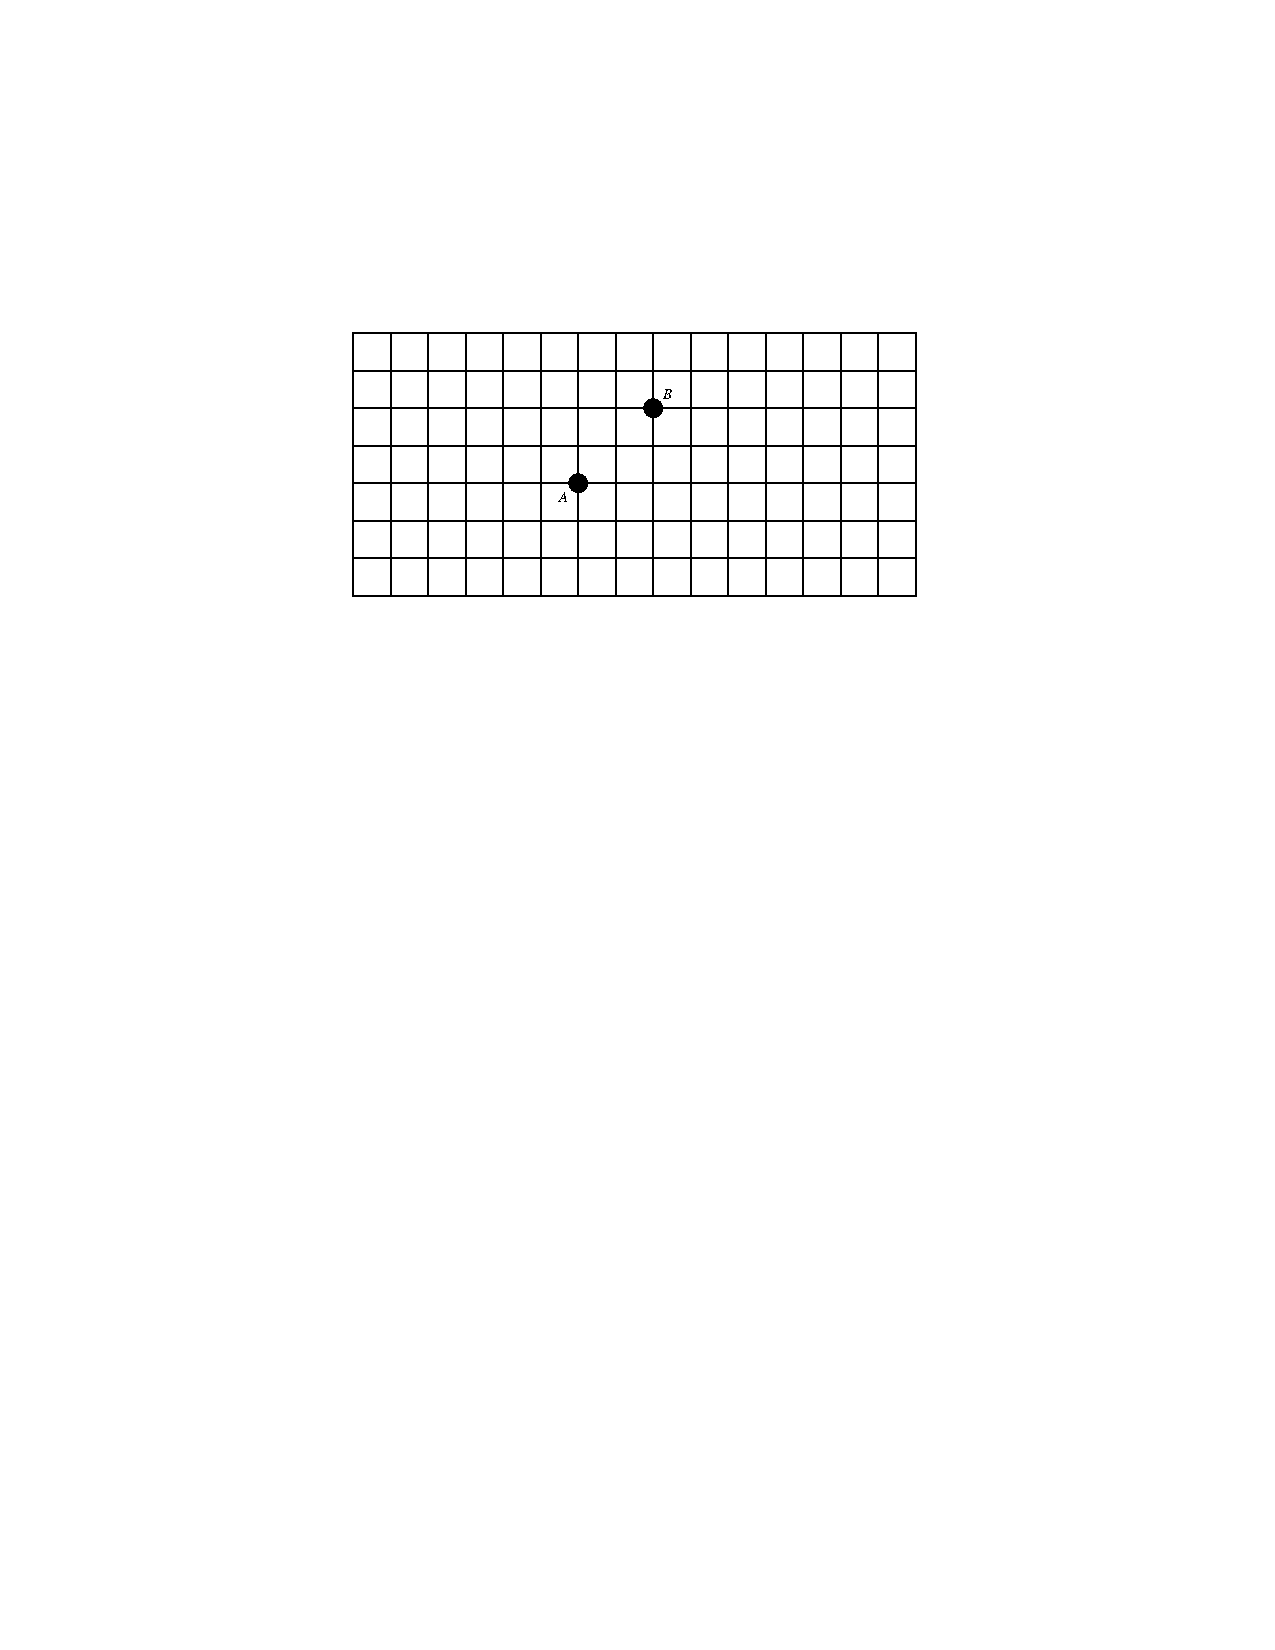
\includegraphics{1166finalmidset.pdf}
\]
\begin{enumerate}
\item Sketch the City Geometry midset of these two points.  
\item Suppose that $A=(0,0)$ and $B=(2,2)$.  Using taxicab distance in City Geometry, write an equation that must be satisfied by any point $(x,y)$ that is in the midset of $A$ and $B$.  
\item Explain the connection between the geometry in part (a) and the algebra in part (b) for the case $x > 2$ and $y < 0$.  
\end{enumerate}
\end{prob}

\begin{prob}
Use coordinate constructions to derive the formula for the parabola
whose focus is the point $(-3,-4)$ and whose directrix is the line $y
= 2$. Show your work. Note, you should use the Euclidean distance
formula, and your final answer should start with ``$y = $''.  
\end{prob}

\begin{prob}
Comparing Celsius and Fahrenheit.  
\begin{enumerate}
\item Water freezes at $0^\circ$ C, which is $32^\circ$ F.  Water boils at $100^\circ$ C, which is $212^\circ$ F.  Use this information to derive a Celsius to Fahrenheit conversion formula.  
\item Suppose the temperature of a model house increases from $24^\circ$ C to $30^\circ$ C, which seems to be a $25\%$ increase.  Convert these temperatures to Fahrenheit and compute the percent change in degrees Fahrenheit. 
\item Use your conversion formula to explain why the percent changes are not the same in Fahrenheit as in Celsius.  
\end{enumerate}
\end{prob}


\begin{prob}
Surface area of a cylinder.
\begin{enumerate}
\item Derive and explain a formula for the surface area of a right cylinder of radius of radius $r$ and height $h$.  
\item Assuming the radius is fixed, how does the surface area vary with the height?  In other words, what kind of function is it?  Explain briefly.  
\item Assuming the height is fixed, how does the surface area vary with the radius?  Explain briefly. 
\end{enumerate}
\end{prob}

\begin{prob}
Volume of a cylinder.
\begin{enumerate}
\item Derive and explain a formula for the volume of a right cylinder of radius of radius $r$ and height $h$.  
\item Assuming the radius is fixed, how does the volume vary with the height?  In other words, what kind of function is it?  Explain briefly.  
\item Assuming the height is fixed, how does the volume vary with the radius?  Explain briefly. 
\end{enumerate}
\end{prob}


\begin{prob}
Standard televisions usually have an aspect ratio (width:length) of 4:3.  Wide-screen televisions have an aspect ratio of 16:9.  Brad's first wide-screen television was a 36 inch (diagonal) model.  Although the new television was clearly wider than the 27 inch (diagonal) standard television it replaced, he was surprised that it did not seem taller than the old television.  Which television was actually taller or shorter?  By how much?  Explain your reasoning.   
\end{prob}

\begin{prob}
Given an equation of a line in standard form, $ax+by=c$:  
\begin{enumerate}
\item Find an efficient way to write down an equation of a perpendicular line through the point $(p,q)$.  
\item Explain why efficient the method works. 
\end{enumerate}
\end{prob}

\begin{prob}
Below is a figure that illustrates part of Euclid's proof of the Pythagorean Theorem.  You may assume the following: 
\begin{itemize}
\item All  angles that appear to be right angles are indeed right.
\item $FB=BA$ and $BD=BC$. 
\item $\triangle ABD \cong \triangle FBC$.  
\end{itemize}
\[
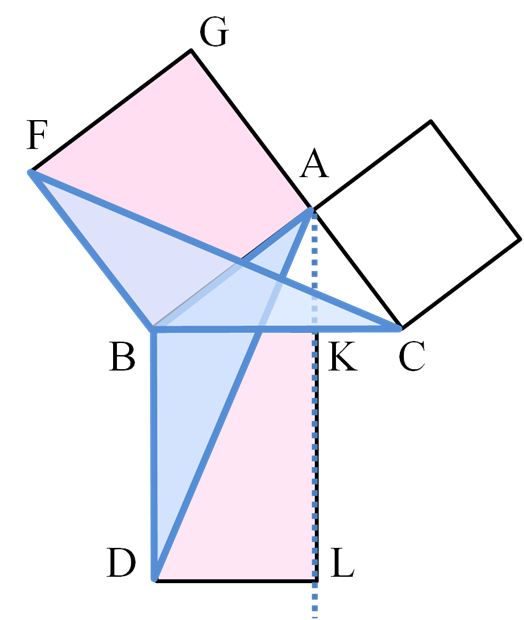
\includegraphics[scale=0.25]{../graphics/Euclid_Pythagorean_theorem3.PNG}
\]
\begin{enumerate}
\item Why is the area of $\triangle KBD$ (not drawn) equal to the area of $\triangle ABD$?
\item Why is the area of $\triangle FBC$ equal to the area of $\triangle FBA$ (not drawn)?
\item Explain briefly why the area of rectangle $KBDL$ equal to the area of rectangle $FBAG$.
\item Now explain how to complete the proof of the Pythagorean theorem.  \end{enumerate}
\end{prob}


%\begin{prob}
%Using the picture below, prove that if two non-vertical lines are perpendicular, the product of their slopes is $-1$.   You may assume that $x$ and $y$ are horizontal and vertical axes, respectively; that lines $j$ and $k$ are perpendicular and that $j$ has positive slope; that the segments of length $a$ and $c$ are vertical and collinear; and that the segment of length $b$ is horizontal.   
%$$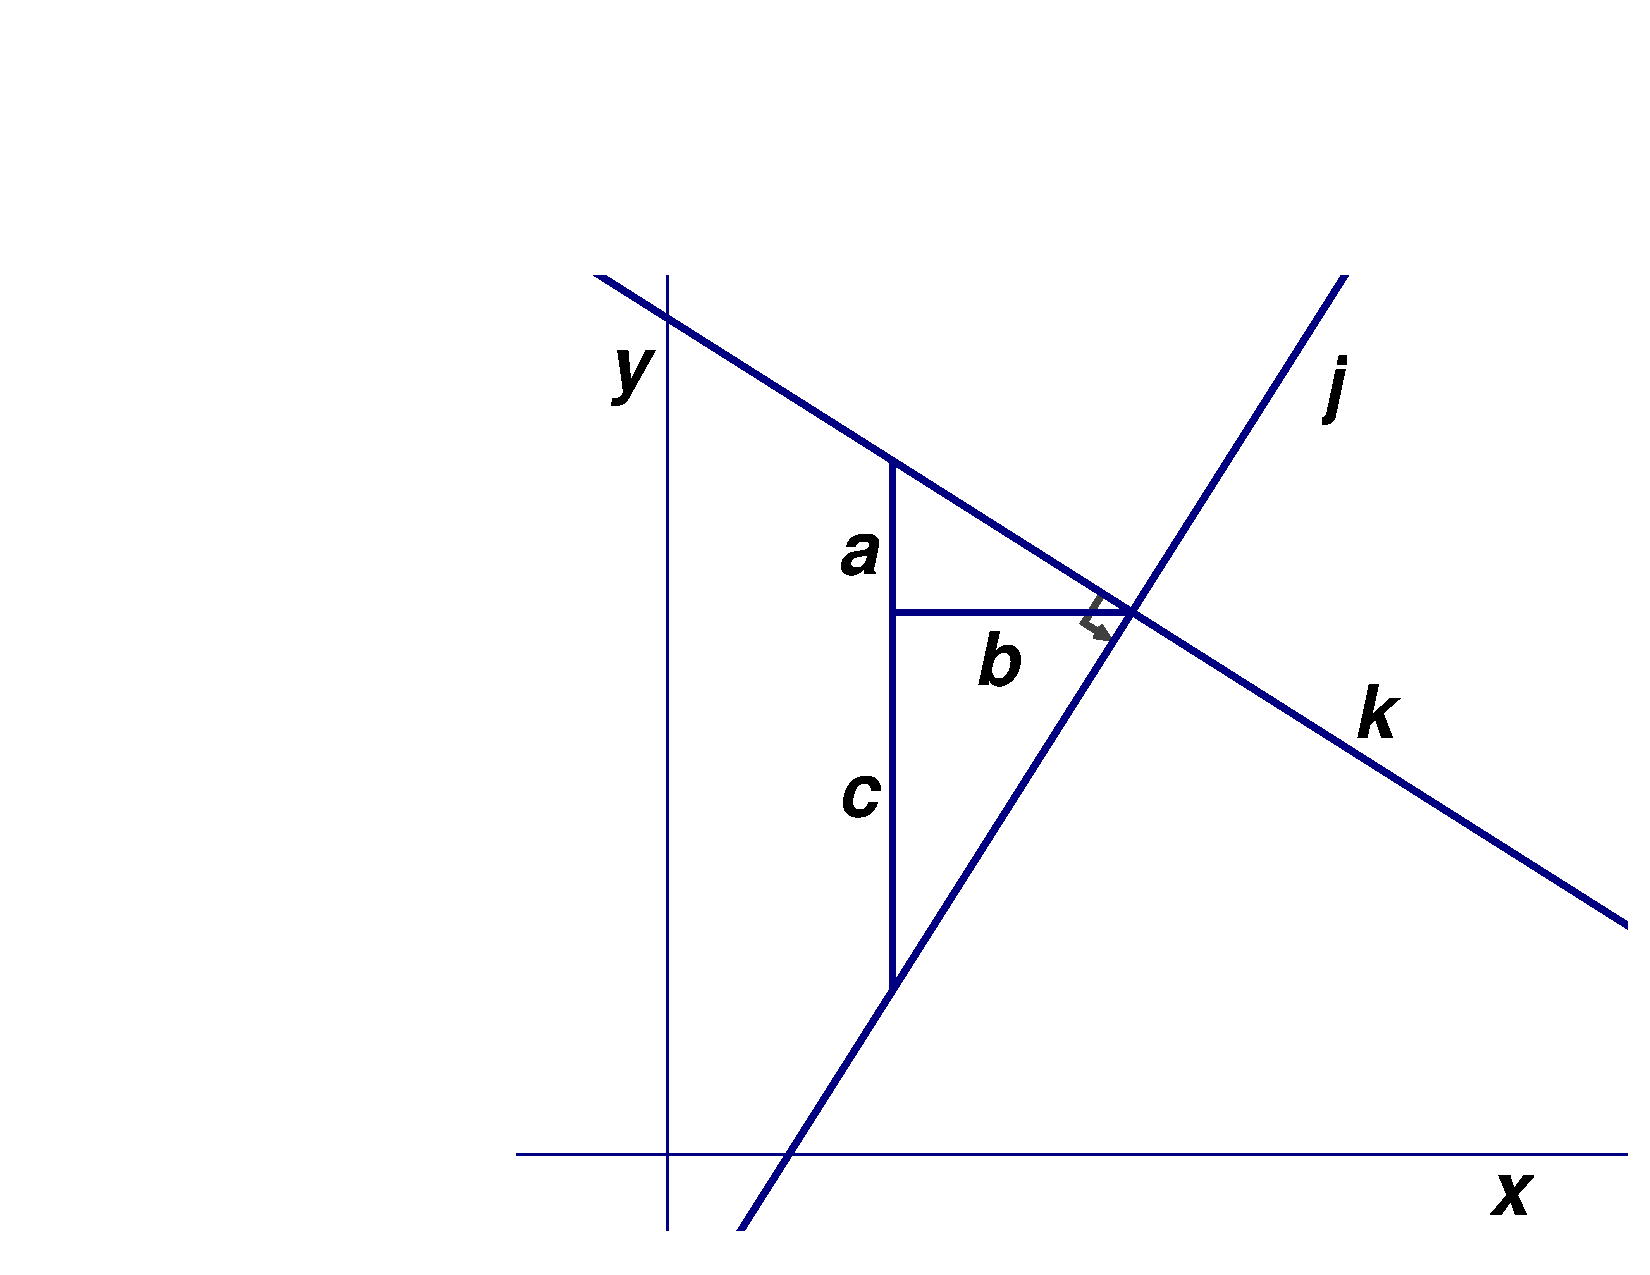
\includegraphics[width=2.5in]{../graphics/perpendicularSlopes.pdf}$$
%\end{prob}

%\subsection*{Questions to be added}
%\begin{enumerate}
%\item Vertex of parabola, completing the square
%\item Trigonometry
%\item Reason with letters.
%\item Solve for different letters.
%\item Different units, measurement
%\item number of solutions 
%\end{enumerate}


\newpage

\section{Math 4407 Exam Review}
The exam will sample from Chapters 1 -- 4 and Activities 1--32 and 38 of your course notes.  Exam problems will focus on Euclidean geometry.  In a few of the problems, you will be asked \emph{to compare the Euclidean result to spherical or hyperbolic geometry and to explain your reasoning.}  
\subsection{Review Ideas}

\begin{itemize}\itemsep0em
\item Be able to state definitions of commonly used terms, such as 
\begin{itemize}
\item Perpendicular line, parallel line, line segment, ray, angle, circle
\item Concurrent, collinear
\item Equilateral, equiangular, and regular polygons
\item Acute, obtuse, and right angles and triangles; isosceles and scalene triangles
\item Straight, complementary, and supplementary angles
\item Trapezoid (inclusive and exclusive), parallelogram, rhombus, rectangle, square, kite
\item Median, perpendicular bisector, angle bisector, altitude
\item Centroid, circumcenter, incenter, orthocenter
\item Chord, arc, arc measure, central angle, inscribed angle, tangent
\end{itemize}
\item Be able to perform standard constructions and explain why they work. 
\item Be able to draw (careful) figures satisfying particular conditions.  
\item Be able to explain key concepts such as area and angle.   
\item Be able to state precisely the triangle congruence criteria. 
\item Know the properties of various special quadrilaterals and be able to prove them.  
\item Know the various centers of a triangle, how to construct them, and whether they can lie outside the triangle.  
\item Be able to state key theorems and prove them in at least two (2) ways, especially:  
\begin{itemize}
\item Isosceles triangle theorem and its converse
\item Pythagorean theorem and its converse
\item The angle sum of a triangle 
\end{itemize}

\item Know the distinction between synthetic and analytic geometry.
\item Know the basic rigid motions, what is required to specify them, and their properties. 
\item Know what it means to say that transformations of the plane are functions.  
\item Know how to define congruence in terms of basic rigid motions. 
\item Know how to define similarity in terms of dilations and basic rigid motions.  
\item Know and be able to use criteria for congruence and similarity of triangles.  
\item Know how to use transformations  to describe symmetries of figures, including tessellations.  
%\item Know the focus and directrix definition of parabola and be able to use it in both synthetic and analytic geometry.
\item Know the definition of circle and be able to use it in both synthetic and analytic geometry.
\item Be aware of assumptions underlying Euclidean geometry and how those assumptions can be different in other geometries (such as spherical geometry).  
\item Use similarity to find missing lengths by reasoning from the scale factor or from within-figure comparisons.   
\item Understand right-triangle trigonometry as similarity, and use trigonometry to solve problems.  (See activity A.27 for a review.)
%\item Reason about length, area, and volume in similarity situations.  How are rep-tiles related to this question?  
%\item Use shearing and Cavalieri's principle to reason about area and volume.  
%\item If you know the area of a rectangle, what can you say about its perimeter?  What about more general figures?  
%\item If you know the perimeter of a rectangle, what can you say about its area?  What about more general figures? 

\end{itemize}

\subsection*{Review Problems}
\begin{prob}
Describe Euclid's (compass and straightedge) construction for an equilateral triangle, and explain
why it works.
\end{prob}

%\begin{prob}
%Use the picture below to show that a pair of medians intersects at a point 2/3 of the way from the vertex to the opposite side.  Then use that fact to argue that the three medians must be concurrent.  
%$$\includegraphics[width=2.5in]{../graphics/median1.pdf}$$
%\end{prob}

\begin{prob}
Prove that the points on an angle bisector are \emph{exactly those} that are equidistant from the sides of the angle. 
\end{prob}

\begin{prob}
Construct a $30$-$60$-$90$ right triangle. Explain the steps in your
  construction and how you know it works.
\end{prob}

\begin{prob}
Construct a $45$-$45$-$90$ right triangle. Explain the steps in your
  construction and how you know it works.
\end{prob}

\begin{prob}
Where is the orthocenter of a right triangle?  Explain your reasoning.  What about the circumcenter?  Again, explain your reasoning. 
\end{prob}

\begin{prob}
Show that, given any three non-collinear points in the Euclidean plane, there is a unique circle passing through the three points.
\end{prob}

\begin{prob}
Prove: A radius that is perpendicular to a chord bisects the chord. 
\end{prob}

\begin{prob}
Prove:  A radius that bisects a chord is perpendicular to the chord. 
\end{prob}

\begin{prob}
Given a circle, give a construction that finds its center.
\end{prob}

\begin{prob}
State and prove a condition about the opposite angles of any quadrilateral that is inscribed in a circle.  
\end{prob}

\begin{prob}
Construct a tangent line from a point outside a given circle to the circle.
\end{prob}

\begin{prob}
Give an informal derivation of the relationship between the circumference and area of a circle. 
\end{prob}

\begin{prob}
Prove:  If a quadrilateral is a parallelogram, then opposite sides are congruent.
\end{prob}

\begin{prob}
Prove:  If opposite sides of a quadrilateral are congruent, then it is a parallelogram.
\end{prob}

\begin{prob}
Claim:  The diagonals of a rhombus are perpendicular. 
\begin{enumerate}
\item Prove the claim. 
\item State the converse of the claim. 
\item Is the converse true?  If so, prove it.  If not, ``salvage it'' to make a true statement, and prove it.  
\end{enumerate}
\end{prob}


\begin{prob}
Draw an arbitrary convex quadrilateral.  Form a second quadrilateral by connecting the midpoints of the sides 
of the first quadrilateral.  You will notice that the second quadrilateral is a special quadrilateral. Make a conjecture about the second quadrilateral and prove it.  
\end{prob}

\begin{prob}
The following picture shows a triangle that has been folded
  along the dotted lines:
\[
\includegraphics{../graphics/origamiPBPTri.pdf}
\]
Explain how the picture ``proves'' the following statements:
\begin{enumerate}
\item The interior angles of a triangle sum to $180^\circ$. 
\item The area of a triangle is given by $bh/2$. 
\end{enumerate}
\end{prob}

%\begin{prob}
%The figure below illustrates a construction given an angle $\theta$ and a segment $\overline{AB}$.  Line $\overleftrightarrow{DE}$ is the perpendicular bisector of $\overline{AB}$, and $\overleftrightarrow{BE}$ is perpendicular to $\overrightarrow{BC}$, as marked.  
%\[
%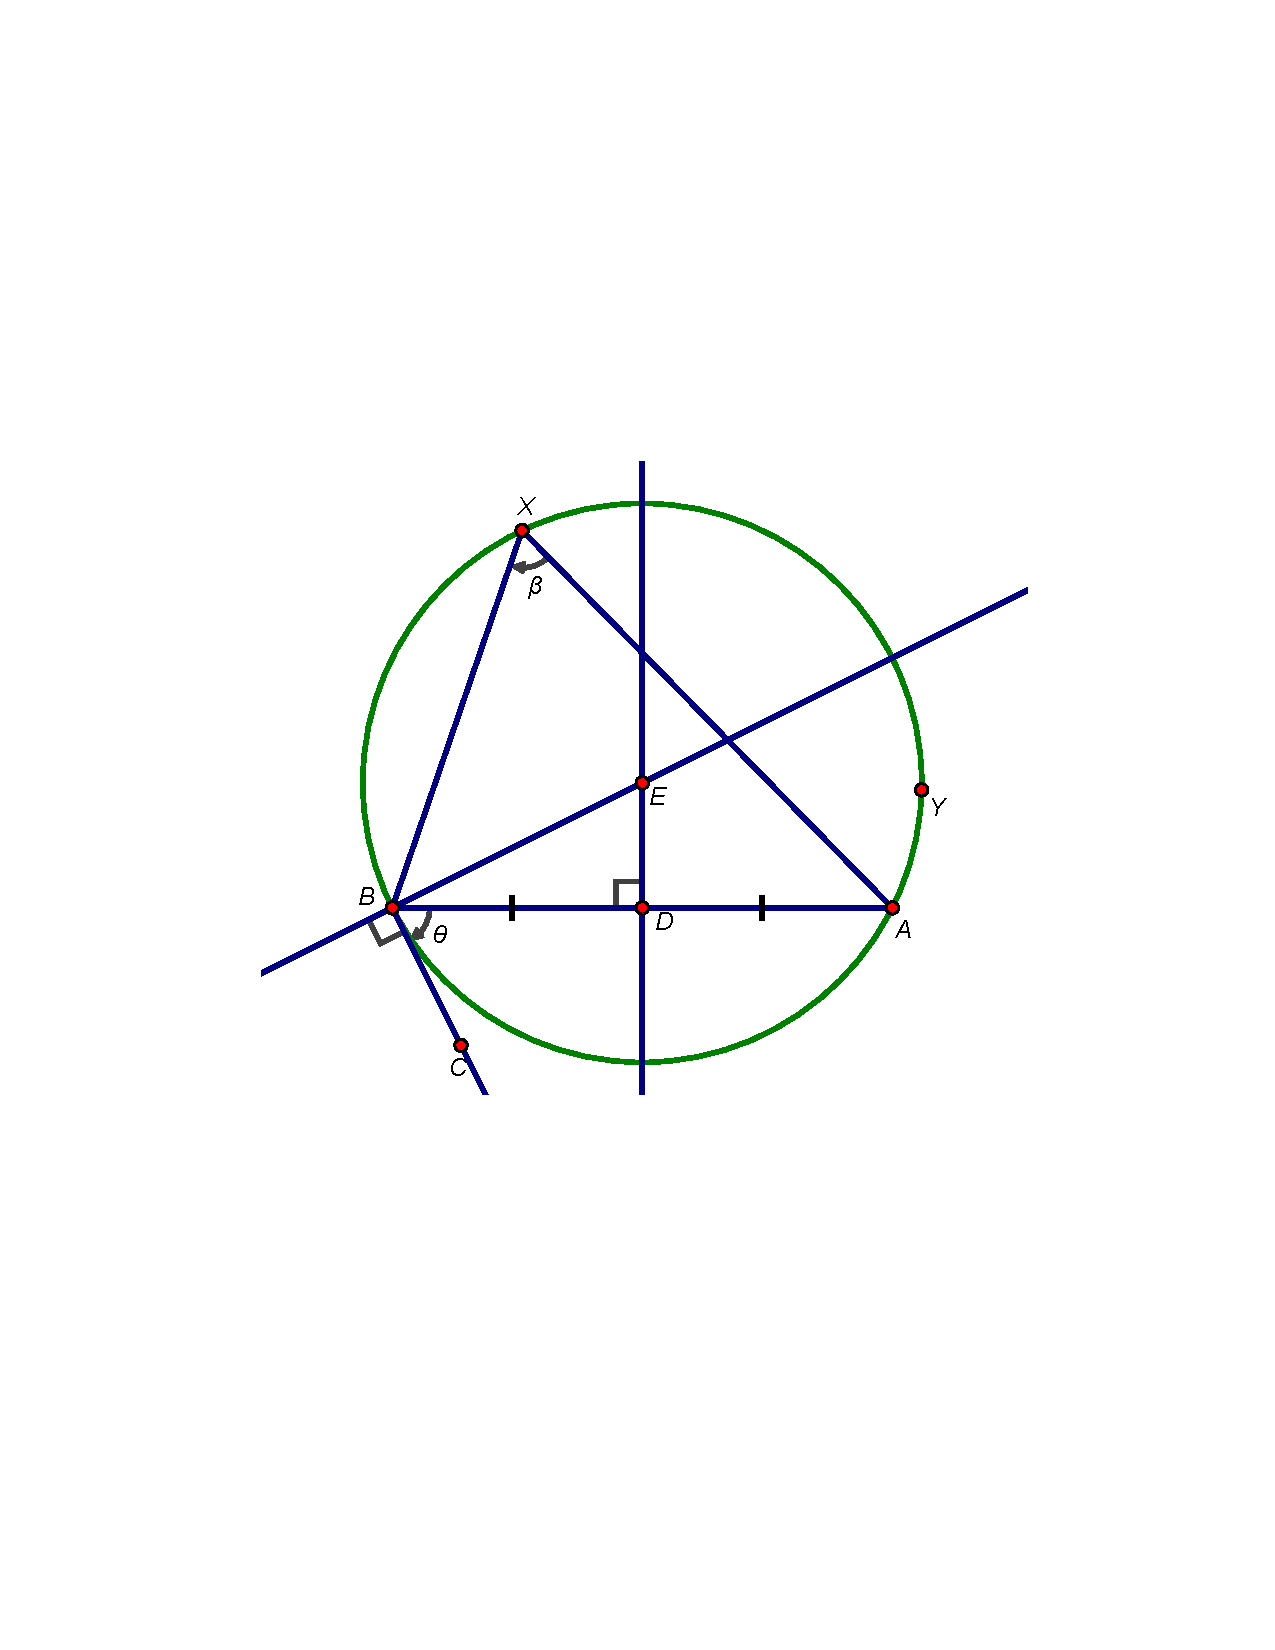
\includegraphics[scale=0.5]{../graphics/trickyConstruction}
%\]
%\begin{enumerate}
%%\item Mark the diagram and state what must be true about the construction so that $\angle\alpha=\angle\beta$. 
%\item Prove that $\angle\theta=\angle\beta$. 
%\item What will happen to $\angle\beta$ if point $X$ is moved over to point $Y$?
%\end{enumerate}
%\end{prob}

%
%\begin{prob}
%During a solar eclipse we see that the apparent diameter of the Sun and Moon are nearly equal. If the Moon is around 240,000 miles from Earth, the Moon's diameter is about 2000 miles, and the Sun's diameter is about 865,000 miles how far is the Sun from the Earth?
%\begin{enumerate}
%\item Draw a relevant (and helpful) picture showing the important points of this problem.
%\item Write an expression that gives the solution to this problem---show all work.
%\end{enumerate}
%\end{prob}
%
%\begin{prob}
%David proudly owns a 42 inch (measured diagonally) flat screen
%  TV. Michael proudly owns a 13 inch (measured diagonally) flat screen
%  TV. Dave sits comfortably with his dog Fritz at a distance of 10
%  feet. How close must Michael sit from his TV to have the ``same''
%  viewing experience?  Explain your reasoning.
%\begin{enumerate}
%\item Draw a relevant (and helpful) picture showing the important
%  points of this problem.
%\item Solve this problem, and be sure to explain your reasoning.
%\end{enumerate}
%\end{prob}

%\begin{prob}
%A typical adult male gorilla is about 5.5 feet tall and weighs about 400 pounds. Suppose King Kong was about 22 feet tall and proportioned like a typical adult male gorilla.
%\begin{enumerate}
%\item Write an expression that approximates King Kong's weight. Briefly explain your reasoning.
%\item The circumference of the neck of a typical adult male gorilla is 36 inches. Approximately what would be the circumference of King Kong's neck? Briefly explain your reasoning.
%\item Suppose an Ohio State sweatshirt for a typical adult male gorilla requires 3 square yards of fabric.  Approximately how much fabric would be required for an Ohio State sweatshirt for King Kong?  Briefly explain your reasoning.
%\end{enumerate}
%\end{prob}
%
%\begin{prob}
%Brenah is drinking fruit punch from a glass shaped like an inverted cone.  Suppose the glass has a height 5 in. and a base of radius 2 in.  What is the volume of the glass?  What is the height of the fruit punch when the glass is half full?  Generalize your result for any glass shaped like an inverted cone.  
%\end{prob}

%\begin{prob}
%A cup has a circular opening, a circular base, and circular cross sections at every height parallel to the base.  The opening has a diameter of 9 cm, the base has a diameter of 6 cm, and the cup is 12 cm high.  
%What is the volume of the cup?  Explain your reasoning.  
%If the cup is filled to half its height, what fraction of the cup's volume is filled?  Explain your reasoning.  
%\end{prob}

\begin{prob}
Suppose you use a photocopier to enlarge a figure to 125\% of its original size.  What is the scale factor of the enlargement?  What happens to areas under the enlargement?  If you lost the original figure, what reduction percentage would you use on the enlargement to create a figure congruent to the original?  What is the scale factor for the reduction?  
\end{prob}

\begin{prob}
Explain how the following picture ``proves'' the Pythagorean Theorem.
\[
\includegraphics[scale=0.75]{../graphics/pbpdilation.pdf}
\]
\end{prob}

%\begin{prob}
%Here is a right triangle, note it is \textbf{not} drawn to scale:
%\[
%\includegraphics{../graphics/origamiSimQ.pdf}
%\]
%Solve for all unknowns in the following cases.
%\begin{enumerate}
%\item $a = 3$, $b = ?$, $c = ?$, $d = 12$, $e = 5$, $f = ?$
%\item $a = ?$, $b = 3$, $c = ?$, $d =8$, $e = 13$, $f = ?$
%\item $a = 7$, $b = 4$, $c = ?$, $d =?$, $e = 11$, $f = ?$
%\item $a = 5$, $b = 2$, $c = ?$, $d =6$, $e = ?$, $f = ?$
%\end{enumerate}
%In each case explain your reasoning.
%\end{prob}

%\begin{prob}
%Describe a general (and foolproof) way of demonstrating that any two parabolas are similar.
%\end{prob}
%
%\begin{prob}
%Construct a tangent line from a point outside a given circle to the circle.
%\end{prob}
%
%\begin{prob}
%Explain how the formula for the volume of a sphere follows from the formula for the volume of a cone and Cavalieri's Principle.
%\end{prob}
%

\begin{prob}
Given a figure and a rotation of that figure, find the center and angle of rotation.  
\end{prob}

\begin{prob}
In the figure below  $O$ is the center of the circle, $\overline{XY}$ is a diameter, $a = PX$, $b=PY$, and $c=PZ$.  
$$\includegraphics[scale=0.6]{../graphics/means}$$
\begin{enumerate}
\item Show that $c=\sqrt{ab}$.  
\item Use the figure to explain the Arithmetic-Geometric Mean Inequality: $\frac{a+b}{2} \ge \sqrt{ab}$.  
%\item Why is this called the Arithmetic-Geometric Mean Inequality?  
\end{enumerate}
\end{prob}

%\begin{prob}
%If the perimeter of a rectangle is 20 feet, what is the most one can say about the rectangle's area?  If the perimeter of any simple closed 2-dimensional shape is 20 feet, what is the most anyone can say about its area?
%\end{prob}
%
%\begin{prob}
%If the surface area of a rectangular prism is 20 square feet, what is the most one can say about the prism's volume?  If the surface area of any simple closed 3-dimensional shape is 20 square feet, what is the most one can say about its volume? 
%\end{prob}

%\begin{prob}
%Why do cute furry animals curl up to stay warm in the winter?  Why are most ugly desert reptiles long and skinny?
%\end{prob}
%
%\begin{prob}Simple closed curve A is contained entirely inside simple closed curve B.  
%\begin{enumerate}
%\item True or False:  The area enclosed by A is less than the area enclosed by B. Explain
%\item True or False:  The perimeter of A is less than the perimeter of B. Explain.  
%\end{enumerate}
%\end{prob}

%\begin{prob}
%Is it correct to say that ``area is length times width''?  Think about what these three quantities mean.  When would it be correct in the numerical sense and why?  (Make sure you use the meaning of multiplication.)   
%\end{prob}

%\begin{prob}
%The apothem of a regular polygon is defined to be the shortest distance from the center of the polygon to an edge.
%\begin{enumerate}
%\item There is a nice relationship between the apothem, perimeter, and area for a regular polygon.  See if you can find it. (Hint:  Split the polygon into congruent triangles from its center and find the area of the polygon in terms of the apothem and perimeter.)  You can assume you know the area of a triangle $=\frac{1}{2}$(Length of Base)(Length of Height).
%\item What does this result say about the area of a circle?  Explain. (Assume you know the circumference of a circle is $2\pi(radius)$.)
%\end{enumerate}
%\end{prob}

%\begin{prob}
% Is it correct to say that ``volume is length times width times height''? What must be true about a figure so that the numerical volume can be more easily measured by ``area times height''?
%\end{prob}
%
%\begin{prob}
%Are there figures for which there is no formula for measuring length, area, and volume?  Explain.  What does your answer to this question imply about the teaching of geometric measurement?
%\end{prob}
%
%\begin{prob}
%Convert 25 yards to meters (and 25 meters to yards) using ``2.54 cm in each inch'' as the only Metric-English unit conversion.  Now convert 25 square yards to square meters and 25 square meters to square yards.  Do the same with cubic yards and cubic meters.
%\end{prob}

%\begin{prob}
%In track and field, 1600 meters is often called the ``one mile,'' but this is not exactly correct.  Is 1600 meters longer or shorter than one mile?  By how much?  
%\end{prob}
%
%\begin{prob}
%Felicia and Wesley are neighbors.  The common boundary between their properties consists of two line segments, as shown below.  
%$$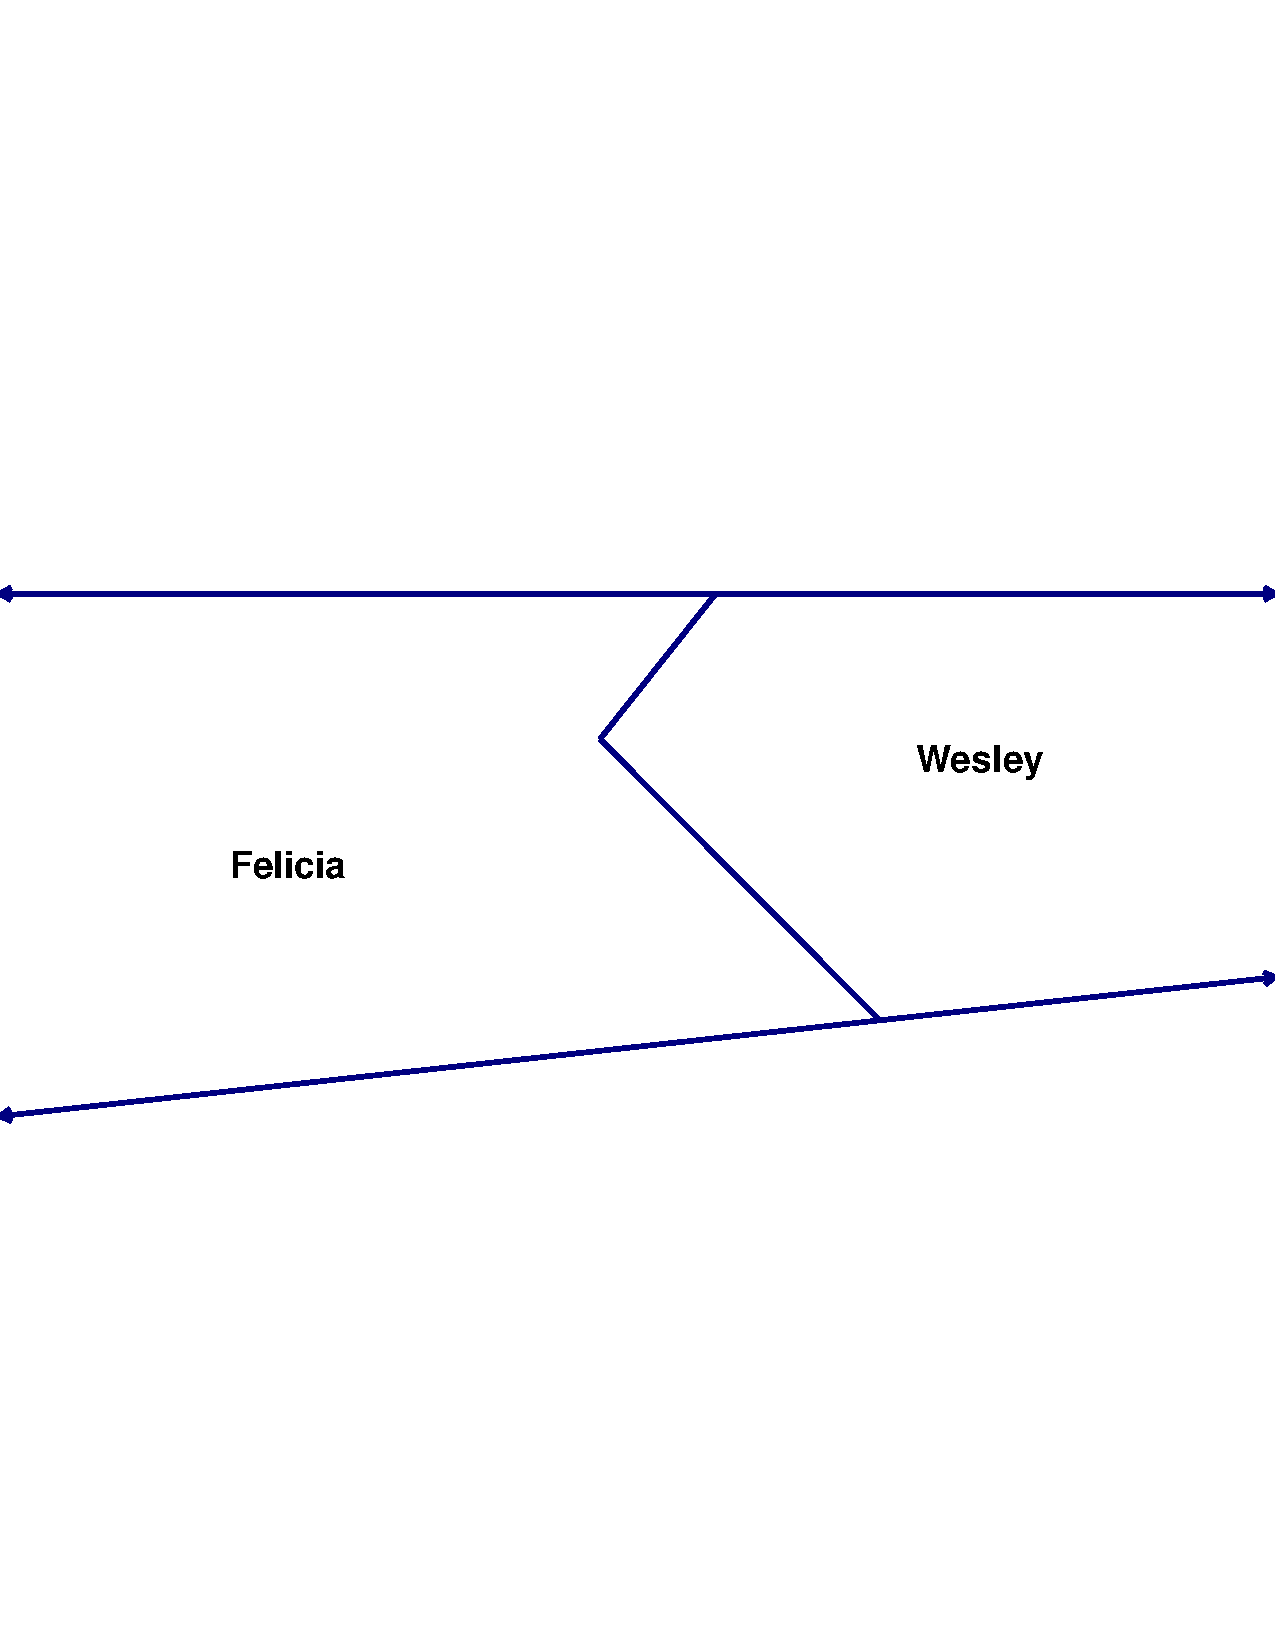
\includegraphics[scale=0.38]{../graphics/TIMSS}$$
%They would prefer their common boundary to be a single straight segment.  How might they change their boundary so that they 
%each have the same area as they have now?  
%\end{prob}
%
%\begin{prob}
%Write an equation of the line through $(2,4)$ parallel to $5x-3y=1$.  
%Now write an equation of the line through $(x_1,y_1)$ parallel to $ax+by=c$. 
%\end{prob}
%
%\begin{prob}
%Write an equation of the line through $(2,4)$ perpendicular to $5x-3y=1$.  
%Now write an equation of the line through $(x_1,y_1)$ perpendicular to $ax+by=c$. 
%\end{prob}

%\begin{prob}
%Intersections of lines.  
%\begin{enumerate}
%\item Find the intersection of the lines $2x-3y=4$ and $3x-5y=3$.  
%\item Find the intersection of the lines $2x-3y=4$ and $-4x+6y=-8$.
%\item Find the intersection of the lines $2x-3y=4$ and $-4x+6y=5$.
%\item How might you have predicted in advance how many solutions to expect for each previous system of equations?
%\item Use algebra to help explain why lines intersect in zero, one, or infinitely many points.  (You know this geometrically, of course.  Here you demonstrate how algebra gives the same result.)  Indicate clearly the algebraic conditions
%for which you get zero, one, or infinitely many points.  
%\end{enumerate}
%\end{prob}

%\begin{prob}
%Suppose you have a rectangle with vertices at $(0,0)$, $(a,0)$,
%$(a,b)$ and $(0,b)$. Use algebra to prove that the diagonals have the
%same length.
%\end{prob}

%\begin{prob}
%Use a general (non-special) triangle to explain why every triangle is a rep-4-tile.  
%Use the same triangle to explain why every triangle tessellates the plane.  Then use your tessellation to explain why every triangle is a rep-$n^2$-tile for any positive integer $n$. 
%\end{prob}

\begin{prob} 
Concurrency of angle bisectors. 
\begin{enumerate}
\item For an arbitrary triangle, draw carefully to demonstrated that the angle bisectors of a triangle are concurrent at the incenter.   
\item Prove that the angle bisectors of a triangle are concurrent.  (Hint:  You may use the result, proved in lecture, that the points on an angle bisector are exactly those that are equidistant from the sides of the angles.)  
\end{enumerate}
\end{prob} 

\begin{prob}
Explain how the ASA congruence criterion follows from the definition of congruence in terms of rigid motions. Be sure to indicate, using the two given angles and the included side, why the sequence of rigid motions guarantees triangle congruence.
\end{prob}


\begin{prob}
Find the intersection of the lines
\begin{align*}
x_1(t) &= -6 + 9t & x_2(t) &= 3+t \\
y_1(t) &= 3-2t &  y_2(t) &= -4-2t 
\end{align*}
If $(x_1(t),y_1(t))$ gives the position of $\mathrm{jogger}_1$ and
$(x_2(t),y_2(t))$ gives the position of $\mathrm{jogger}_2$, what is
the significance of the point of intersection of these lines, from the
perspective of the joggers?
\end{prob}

\begin{prob}
A bug moves according to the following parametric equations, where t is measured in seconds and $x$ and $y$ are measured in centimeters:  $x = 2t^2$, $y = t-2$.  (Suppose $t$ can be any real number.)   
\begin{enumerate}
\item Describe the path of the bug.  
\item Is the bug's position a function of time?  
\item On the path, is $y$ a function of $x$?  
\item Is $x$ a function of $y$?  
\item If you know one of $x$, $y$, or $t$, can you determine the other two?  How does this question relate to the previous two questions?  
\item In school mathematics, students are often given a graph and asked, ``Is it a function.''  Explain why this is a poor question.  What better questions could you ask?  
\end{enumerate}
\end{prob}

%%\subsection{Absolute Value, Distance, and City Geometry}
%\begin{prob}
%Consider the following equations:  
%\setlength{\arraycolsep}{12pt}
%\setlength{\extrarowheight}{3pt}
%\[
%\begin{array}{cccc}
%x^2-y^2=0    &   x^2=y^2   &   |y|=|x|   &   y= \pm x \\
%(x-y)(x+y)=0  &   x= \pm y   &   y = \pm|x|   & x = \pm|y|
%\end{array}
%\]
%\begin{enumerate}
%\item Which equations are equivalent to which other equations?  Say how you know.  (Be sure to state what it means for the equations to be equivalent.)
%\item For each set of equivalent equations, graph the solution set, and describe how each of the equations provides a different way about thinking about that solution set.  
%\end{enumerate}
%\end{prob}


\end{document}
